\documentclass[a4paper, 12pt]{article}

%% подключаем стандарт библиографии
\bibliographystyle{gost71u} 

%% for envirovemt "abstract" in class book
%%\newenvironment{abstract}{}{}
\usepackage{abstract}

%% подключаем преамбулу, в ней содержатся подключение всех необходимых пакетов
%%% Работа с русским языком
\usepackage{cmap}			 % поиск в PDF
\usepackage{mathtext} 		 % русские буквы в формулах
\usepackage[T2A]{fontenc}	 % кодировка
\usepackage[utf8]{inputenc}	 % кодировка исходного текста
\usepackage[russian]{babel}	 % локализация и переносы

%%% Пакеты для работы с математикой
\usepackage{amsmath,amsfonts,amssymb,amsthm,mathtools}
\usepackage{icomma}

%% Номера формул
%\mathtoolsset{showonlyrefs=true} % Показывать номера только у тех формул, на которые есть \eqref{} в тексте.
%\usepackage{leqno}               % Немуреация формул слева

%% Шрифты
\usepackage{euscript}	 % Шрифт Евклид
\usepackage{mathrsfs}    % Красивый матшрифт
\usepackage[14pt]{extsizes} % Задаем 14 шрифт

%% Поля (геометрия страницы)
\usepackage[left=3cm,right=2cm,top=2cm,bottom=2cm,bindingoffset=0cm]{geometry}

%% Русские списки
\usepackage{enumitem}
\makeatletter
\AddEnumerateCounter{\asbuk}{\russian@alph}{щ}
\makeatother

%% Создание списка литературы
\usepackage{etoolbox}
\makeatletter
\patchcmd{\bibliography}{%
  \chapter*{\bibname}\@mkboth{\MakeUppercase\bibname}{\MakeUppercase\bibname}}{%
  \section{Список литературы}}{}{}
\makeatother

%%% Работа с картинками
\usepackage{caption}
\usepackage{subcaption}
\captionsetup{justification=centering} % центрирование подписей к картинкам
\usepackage{graphicx}                  % Для вставки рисунков
\graphicspath{{images/}{images2/}}     % папки с картинками
\setlength\fboxsep{3pt}                % Отступ рамки \fbox{} от рисунка
\setlength\fboxrule{1pt}               % Толщина линий рамки \fbox{}
\usepackage{wrapfig}                   % Обтекание рисунков и таблиц текстом

%%% Работа с таблицами
\usepackage{array,tabularx,tabulary,booktabs} % Дополнительная работа с таблицами
\usepackage{longtable}                        % Длинные таблицы
\usepackage{multirow}                         % Слияние строк в таблице
\usepackage{diagbox}

%% Красная строка
\setlength{\parindent}{2em}

%% Интервалы
\linespread{1.5}
\usepackage{multirow}

%% TikZ
\usepackage{tikz}
\usetikzlibrary{graphs,graphs.standard}

%% Верхний колонтитул
\usepackage{fancyhdr}
\pagestyle{fancy}

%% Перенос знаков в формулах (по Львовскому)
\newcommand*{\hm}[1]{#1\nobreak\discretionary{}{\hbox{$\mathsurround=0pt #1$}}{}}

%% дополнения
\usepackage{float}   % Добавляет возможность работы с командой [H] которая улучшает расположение на странице
\usepackage{gensymb} % Красивые градусы
\usepackage{caption} % Пакет для подписей к рисункам, в частности, для работы caption*

% подключаем hyperref (для ссылок внутри  pdf)
\usepackage[unicode, pdftex]{hyperref}

\begin{document}
    %% титульник
    \begin{center}
    %% *название института*
    \large\textbf{Министерство образования и науки Российской Федерации \\
    Московский физико-технический институт (национальный исследовательский университет)} \\
    \vspace{1cm}

    %% *факультет/физтех-школа*
    Физтех-школа радиотехники и компьютерных технологий \\

    %% *название базовой кафедры и лаборатории*
    %% в случае ненадобности можно удалить
    Кафедра интеллектуальных информационных систем и технологий \\

    \vspace{4em}

    Выпускная квалификационная работа бакалавра
\end{center}

\begin{center}
    \vspace{\fill}
    %% *название вашей работы*
    \LARGE{Исследование методов классификации движений человека}

    \vspace{\fill}
\end{center}


\begin{flushright}
    \textbf{Автор:} \\
    Студент Б01-815а группы \\
    Токарев Андрей Сергеевич \\
    \vspace{2em}
    \textbf{Научный руководитель:} \\
    Ст. Преподаватель \\
    Воронков Илья Михайлович \\
\end{flushright}

\vspace{7em}

\begin{center}
    %% *лого*
    
\includegraphics[width=100 pt]{MIPT_logo.jpg}\\
    Москва \the\year{}
\end{center}

% выключаем отображение номера для этой страницы (титульник)
\thispagestyle{empty}

\newpage
\setcounter{page}{2}
\fancyfoot[c]{\thepage}
%% *надпись над верхним колонтинулом*
%% в случае ненадобности можно удалить
\fancyhead[L]{Исследование методов классификации движений человека}
\fancyhead[R]{}
    %% аннотоция
    \begin{abstract}

    \begin{center}
        \large{Исследование методов классификации движений человека} \\
    \large\textit{Токарев Андрей Сергеевич} \\[1 cm]
    \end{center}
    
	\begin{large}   
   После достижения результатов в задаче сегментации человека и отслеживании его на видео стало интересна возможность оценки занимаемой им позы и ее классификация. Для этого было необходимо научиться распознавать выбранные ключевые точки на теле человека, которые несут информацию о его положении. Некоторые группы исследователей уже добились хороших результатов в данном направлении и двигаются дальше в задачах анализа взаимодействия между людьми и предсказания следующих движений человека.
	\end{large}
  
	\begin{large}   
   В данной работе представлен обзор задачи классификации движений на основе информации о ключевых точках на теле человека, а также приведены технический обзор и исследование систем глубокого обучения для оценки позы на основе публичных наборов данных.
	\end{large}

\end{abstract}
\newpage
    %содержание
    \tableofcontents{}
    \newpage

    \section{Введение}
\label{sec:Chapter0} \index{Chapter0}

В этой части надо описать предметную область, задачу из которой вы будете решать, объяснить её актуальность (почему надо что-то делать сейчас?).
Здесь же стоит ввести определения понятий, которые вам понадобятся в постановке задачи.

\hfill \break
\textbf{\Large 3 Вариант введения.}

Понимание движений человека является необходимой частью нашей жизни. При общении людьми часто используется жестикуляция, так как это помогает выражать чувства, эмоции и доносить свои мысли до окружающих . Из анализа позы человека можно сделать вывод о его состоянии. К примеру, хромота или нахождение в неестественном положении говорят о необходимости не только медицинской, но, возможно, и вашей помощи. Ещё можно обратится к психоанализу, а точнее к разделу о языке телодвижений. В нем по позе можно сделать вывод о характере человека или о текущем состоянии, его заинтересованности  в беседе.Также работает распознавание движений. Если мы видим бегущих в панике людей, то наш мозг получает сигнал об опасности и спасает нас. Из приведенных ситуацию   становится  понятно, почему определение позы и классификация движений являются важными аспектами нашей жизни. В связи с развитием информационных технологий, человечество задумалось над выполнением данной задачи с помощью компьютера. Тогда можно будет добавить дополнительный источник информации для  взаимодействия искусственного интеллекта с человеком.

При рассмотрении данной задачи через призму машинного обучения, получим, что нам нужно классифицировать положение человека, данные о котором необходимо каким-то образом получать. Первый способ - надеть на добровольца датчики и, считывая координаты каждого из них, построить на компьютере его позу и, таким образом, восстановить скелет для последующего анализа. Второй способ - искать особые точки на фотографии с помощью компьютерного зрения. Установим камеру и начнем анализировать положение и скелет человека, исходя из картинки. Тогда не придется закупать большое количество датчиков для снятия данных, а нужна будет только камера и вычислительные мощности для работы алгоритмов глубокого обучения. Несмотря на сложность реализации первого варианта, его удобно использовать для подготовки тренировочных датасетов \cite{h36m_pami}.

\hfill \break
Движение - это растянутый во времени процесс. Он анализируется по видеозаписям, каждая из которых представляет собой последовательность кадров. Поэтому первостепенно научиться работать с изображением. Как же собирать данные для модели классификации?

Восстановление скелета (Skeletal Representation), детекция (Pose Detection) и оценка позы (Pose Estimation), распознавание движения (Action Recognition) являются расширением одной задачи: распознавание ключевых точек на теле человека (Key-points Detection). Задачи, которая имеет прикладной смысл не только в связке с классификацией движений. В работе мы будем рассматривать распознавание только на картинке, то есть в 2-х мерном пространстве. Но ведь можно восстанавливать положение человека (скелет человека) в 3-х мерном пространстве \cite{WANG2021103225} \cite{8100086}. Используя генеративные нейронные сети можно воссоздавать не только скелет человека, но и тело человека \cite{Zhang_2017_CVPR}. Объединяя две предыдущие задачи можно получить набор данных из 3-х мерных людей в различных позах. Некоторые исследователи уже пробуют реализовать этот симбиоз на практике \cite{varol17_surreal}.

Если перейти в тематику биологических и медицинских наук, то можно развить данную тему на примере восстановления структуры тканей человека. Получается, мы сможем по фотографии моделировать распределение мышечных, жировых и других тканей в теле человека. Это поможет более детально изучать проблемы персонально, каждого человека и подбирать индивидуальные курсы лечения или диеты.

Восстановление скелета человека поможет спасателям анализировать положение человека под завалами и строить планы по его спасению, имея более детальную информацию. Правда в данном случае необходимо быстродействие алгоритма и очень важно получить изображение человека.

В современном мире, где повсюду слышны разговоры о технологиях дополненной реальности и мета вселенной, найдем ещё одно применение для алгоритмов детектирования позы. Для нахождения в виртуальной вселенной необходимо транслировать человека туда, а значит можно с помощью видеокамер определять положение, восстанавливать скелет и получать итоговое изображение или 3-х мерную модель. Чем-то напоминает фильм "Первому Игроку Приготовиться"{} Стивена Спилберга. Добавим алгоритм генерации аватара вместо реального человека и получим рабочий алгоритм трансляции живого человека в мета вселенную.

\hfill \break
Второй частью работы является задача классификации (Pose Classification), которая использует данные, полученные в первой части. Таким образом, мы построили алгоритм анализа движений человека на статическом изображении. По изображению мы не можем давать оценку поведению человека, но своеобразный "помощник"{} из полученного алгоритма будет хороший. Рассмотрим некоторые идеи применения.

Начать можно с медицины. Восстановление больных после операций, травм и несчастных случаев - это длительный и трудоемкий процесс, требующий постоянного присмотра врача. Если человек учится двигаться, то нужен тренер, который укажет  на ошибки и исправит вас. Решение нашей задачи помогает таким пациентам. Анализ движений может сравнивать человека с эталоном и указывать на ошибки. Также при наблюдении за больным алгоритм может идентифицировать отклонения от нормального поведения и вызвать врача (к примеру увидеть приступы эпилепсии у человека). Это может спасти множество жизней по всему миру, просто вызывая врача в необходимый момент, а также помочь в востановлении.

Также можно выявлять у здорового человека заболевания или дефекты скелета. Можно анализировать сколиоз или сутулость и подсказывать людям, что надо стараться держать спину прямо. Хотя лучше направлять к врачу на консультацию и лечить дефекты позвоночника сразу. Проведя исследование населения, мы получим статистику тех или иных отклонений. Так уже сделали производители кроссовок и с помощью gait-анализа \cite{WHITTLE1996369} помогают выбрать подходящую обувь.

Посмотрим теперь на спорт. Из классификатора можно сделать хорошего судью соревнований в тех видах, где надо различать, отслеживать положения тела. К примеру, GOOGLE придумали использовать классификатор как счетчик подтягиваний, приседаний или отжиманий \cite{counter} и это можно поместить в современный смартфон. Если углубиться дальше, то решение можно обернуть интерфейсом и создать хорошего робота-фитнес-тренера. Ведь настроив камеру смартфона на наблюдение за вами во время тренировки, приложение будет подсказывать вам правильную позу для упражнения и укажет на ошибки, если таковые имеются.

\hfill \break
При развитии моделей в будущем, можно будет найти другие варианты применения технологии классификации движений человека. Можно анализировать поведение группы людей, но для этого надо хорошо восстанавливать скелет нескольких человек на одном изображении \cite{8765346} \cite{https://doi.org/10.48550/arxiv.1807.04067} \cite{fang2017rmpe}. Также есть возможность предсказывать будущие действия человека при изучении уже имеющихся \cite{s20174944}. Если опять затронуть идею генеративных нейронных сетей, то можно генерировать движения человека по заданному начальному условию. Следовательно, можно создавать искусственные видеозаписи или добавлять неигровых персонажей (npc - non-player character) в виртуальную реальность. В медицине можно моделировать восстановление двигательной активности человека или моделирование протезов индивидуально под каждого пациента.

Как можно заметить, применений можно придумать множество - необходимо реализовать проект и получить модель. В текущий момент в мире уже существует какое-то количество решений описанных выше задач. В предложенной вашему чтению работе я рассмотрю некоторые из них, приведу качественную оценку результатам эксперимента и сделаю вывод с определением дальнейшего моего развития в данной теме. (МОЖЕТ СТОИТ УБРАТЬ ПРО МОЕ РАЗВИТИЕ В ДАННОЙ ТЕМЕ?)



\hfill \break
\textbf{\Large 2 Вариант введения. Вроде не законченный.}

После достижение определенных хороших результатов в области детекции объектов на изображениях необходимо было двигаться дальше. Одним из дальнейших направлений стала классификация движений человека с помощью нейронных сетей. Пусть на данный момент уже делаются попытки предсказывать будущие движения человека по предыдущим кадрам видеозаписи (НЕОБХОДИМА ССЫЛКА), но в данной работе мы сфокусируемся на анализе современных методов классификации движений человека. Так как данная задача подразделяется на две части: распознавание ключевых точек на теле человека и классификация движения человека исходя из анализа результатов прошлой части.

Первая часть работы имеет дальнейшее развитие, не связанное с классификацией движений,  в задачу восстановления скелета человека в 3-х мерном пространстве (ССЫЛКА) и в задачу о генерации данных (ССЫЛКА): синтетические люди в 3-х мерном пространстве. Эти задачи могут помочь как ученым в моделировании человеческих поз и их дальнейшем изучении, так и комерческим компаниям в производстве акксессуаров дополненной реальности. А так как в последнее время многие компании развивают идеи виртуальной реальности, то необходимо каким-то образом подгружать человека в виртуальный мир. Одним из способов может стать съемка его через камеру. Представьте через несколько лет виртуальную конференцию в большой компании, где все участники находятся в виртуальном мире через веб-камеру. Интересно, не так ли?

Вторая же часть работы является развитием первой части. Исходя из состояния ключевых точек мы можем построить 2-х мерный скелет, по которому можно проанализировать позу человека. Анализируя позу мы можем сделать вывод о том, какое движение человек выполняет. В этом и состоит анализ движения человека. Развивается данная идея в анализ видео последовательности кадров, в анализ межчеловеческого взаимодействия на картинках и в предсказание будущих движений человека по уже имеющимся.  

\hfill \break
\textbf{\Large 1 Вариант введения.}

В данной работе будет представлен анализ современных систем распознавания ключевых точек на теле человека и классификации движений человека по данным полученным данным. На сегодняшний момент мир довольно сильно развился и требует анализа человеческих действий с помощью искуственного интеллекта. Исходя их таких запросов был сформирован план действий по достижению таких результатов. Такие моменты как переход от 2D картинки  к 3D можелированию скелета человека, сложные позы и разный рост людей решаются в данный момент различными способами, которые будут описаны ниже.

Области применения этой задачи могут быть весьма разнообразные: виртуальная реальность (VR, AR), медицина (восстановлене больных и слежение за их движениями - правильно или неправильно они двигаются), фитнес-приложения (отслеживать правильность выполнения упражнения), производство различных аксессуаров (если человек работает в определенной позе, то можно смоделировать его положение и понять каким образом лучше реализовать инструмент или аксессуар). Одна компания анализировала постановку стопы человека (необходимо добавить ссылку на информацию), чтобы принять решение о выпуске будущей коллекции обуви. Оказалось, что большинство людей заваливают ногу внутрь и из-за этого им лучше покупать специальную обувь. Также можно анализировать правильность выпонения упражнения в спорте, а также вести подсчет повторений на соревнованиях (пожтягивание, отжимание или приседание), ведь если человек не примет верную позу, то повторение не будет засчитано :)

По моим ощущениям данная задача является одной из тех задач, которые помогут упростить жизнь на нашей планете и сделать ее более безопастной и продвинутой. Данная технология поможет во многих отраслях жизни, поэтому я бы хотел продолжить развиваться в области данной задачи.


\newpage %% Введение
    \section{Постановка задачи}
\label{sec:Chapter1} \index{Chapter1}
Здесь надо максимально формально описать суть задачи, которую потребуется решить, так, чтобы можно было потом понять, в какой степени полученное в результате работы решение ей соответствует. Текст главы должен быть написан в стиле технического задания, т.е. содержать как описание задачи, так и некоторый набор требований к решению

Как уже было сказано в главе \ref{sec:Chapter0}, будет произведена классификация движений человека на изображении. Из изображения надо получить данные о принимаемой субъектом позе и классифицировать её на род деятельности человека. Получается мы решаем две задачи: предобработки данных, то есть извлечение расположения ключевых точек на теле человека, и их последующая категоризация. Рассмотрим их по отдельности.


\subsection{Задача распознавания ключевых точек на теле человека}
\label{subsec:Theory of keypoint detection}

Первоначально необходимо понять каким образом можно распознать позу человека, чтобы в дальнейшем взять оттуда информацию для классификации. Человек смотрит на другого человека и анализирует его позицию исходя из данных о его расположении частей тела анализируемого. Получается нам необходимо найти части тела человека, каждая из которых ограничена какими-либо суставами. Последние можно и взять за ключевые точки, которые будут распознаваться моделью. Если соединить выходные данные, то получим рисунок, который большинство из нас рисовало в детстве. (ДОБАВИТЬ РИСУНОК И ВОСCТАНОВЛЕННЫЙ СКЕЛЕТ?)

(Можно сказать, что на сегодня шний момент существует три типа моделей оценки позы человека

Необходимо определиться сколько точек на теле человека необходимо различать. На текущий момент стандартом является топология СОСО (см. \autoref{fig:COCO_topology}), которая включает в себя 17 ориентиров на теле человека \cite{COCO_topology, COCO_dataset}. Данная топология не учитывает расположение ступней и кистей рук, а также рассматривает всего 5 точек на лице человека: нос, два глаза и два уха. Но стандартом многие исследователи не ограничиваются и добавляют дополнительные точки. Приведу два примера:

\begin{enumerate} 
  \item Топология от BlazePose (см. \autoref{fig:BlazePose_topology})\\
  Включает в себя 33 точки расположенные на теле человека. Данная топология представляет собой объединение COCO, BlazeFace \cite{BlazeFace} и BlazePalm \cite{Hands}. В итоге мы получаем дополнительную информацию о направлении стоп и кистей, а также больше понимаем насчет точек на лице. Данная модель расположения точек используется в одноименной модели (BlazePose \cite{BlazePose}) и ориентирована на использование в фитнес приложениях. Также у данной компании есть более развитая модель, которая определяет положение всех пальцев кисти и распознает мимику на лице \cite{Holistic}.
  \item Halpe (см. \autoref{fig:Halpe_topology})\\
  Данная топология - это совместный проект AlphaPose \cite{fang2017rmpe} и HAKE \cite{li2020pastanet}. Представлено две модели: на 26 и на 136 точек. Здесь добавлено рассмотрение ориентации стоп, распознавание шеи, паха и макушки головы. В расширенной модели присутствует ещё 68 точек на лице, а также по 21 на ладонях.
\end{enumerate}

\begin{figure}[h]
\begin{subfigure}[b]{.3\textwidth}
	\centering
	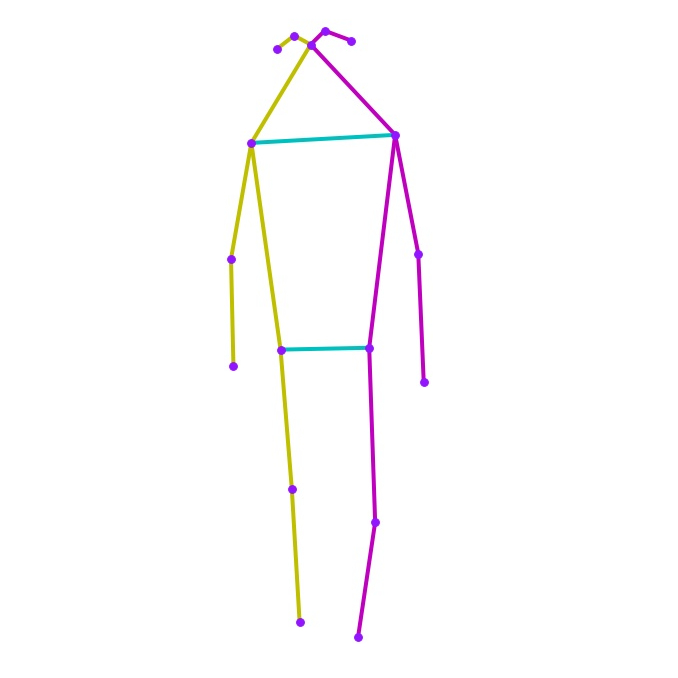
\includegraphics[width=\textwidth]{./images/COCO_topology.jpg}
	\caption{Топология COCO}
	\label{fig:COCO_topology}
\end{subfigure}
\begin{subfigure}[b]{.3\textwidth}
	\centering
    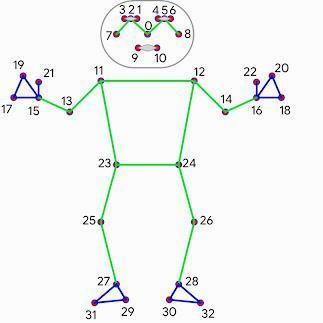
\includegraphics[width=\textwidth]{./images/BlazePose_topology.jpg}
    \caption{Топология BlazePose}
    \label{fig:BlazePose_topology}
\end{subfigure}
\begin{subfigure}[b]{.3\textwidth}
	\centering
    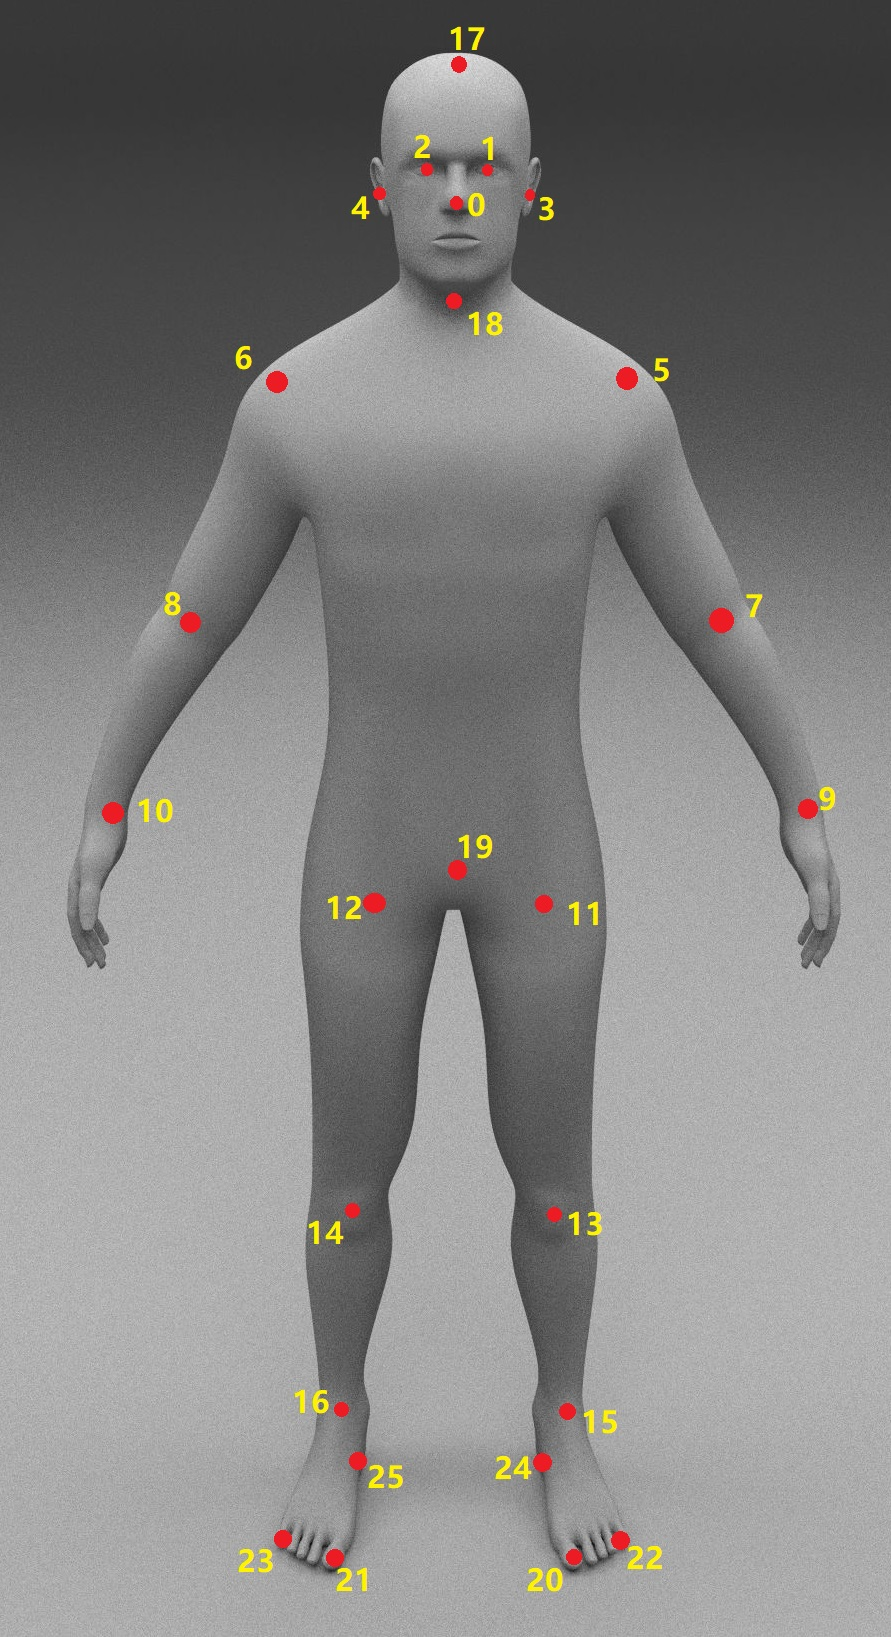
\includegraphics[height=\textwidth]{./images/Halpe_topology.jpg}
    \caption{Топология Halpe}
    \label{fig:Halpe_topology}
\end{subfigure}
    \caption{Примеры расположения точек на теле человека.}
\end{figure}

В итоге мы разобрались с тем что нам необходимо искать в нашей работе и сейчас необходимо понять как это делать. Данная работа проводится в два этапа: 
\begin{enumerate}
	\item Локализация человека и его частей тела
	\item Упорядочивание и распределение суставов в правильном порядке.
\end{enumerate}

В реальном мире мы имеем два подхода к поиску ключевых точек и восстановлению скелета на изображении:
\begin{itemize}
	\item Bottom-up\\
	Когда сначала распознаем точки,  потом собираем их в скелет
	\item Top-down\\
	Сначала происходит локализация людей или объектов, а потом происходит распознование ключевых точек
\end{itemize}

ДУМАЮ ТУТ СТОИТ ПРОДОЛЖИТЬ ИЗ РАЗДЕЛА МНОГО ТЕОРИИ ДЛЯ РАЗБАВКИ РАБОТЫ. О ТОМ КАК ДЕТЕКТИРОВАТЬ И ИСКАТЬ ЭТИ ТОЧКИ. ТАКЖЕ МОЖНО ДОБАВИТЬ ПРО РАЗЛИЧНЫЕ ФУНКЦИИ И ФОРМУЛКИ. ДОЛЖНО ПОЛУЧИТСЯ КРАСИВО И ИНТЕРЕСНО.

\subsection{Задача классификации движений/позы человека}
\label{subsec:Theory of classification}

Полученные координаты ключевых точек можно использовать как признаки для различных классификаторов. Думаю тут не стоит сильно заморачиваться с описанием задачи машинного обучения классификации. Может просто забить, а может расписать и добавить ещё несколько страниц. СПРОСИТЬ У НАУЧРУКА ПРО ДАННЫЙ РАЗДЕЛ!!!
\newpage %% Постановка задачи
    \section{Обзор существующих моделей}
\label{sec:Chapter2} \index{Chapter2}

\subsection{Модели для распознавания ключевых точек на теле человека}
\label{subsec:pose_estimation_models}

В данном разделе будет рассмотрено 6 различных моделей. В \autoref{sec:Chapter4} будут выбраны 4 наиболее удобные в использовании и в обучении и будет проведен эксперимент по оценке данных моделей.

Так же хочется сказать, что, помимо приведенных, есть множество моделей от одиночных авторов, не объединенных в лаборатории \cite{pet_recognition, pet_classification}. Они в основном брали какую-то из представленных ниже моделей и проводили небольшое улучшение.

А теперь перейдем к моделям.

\subsubsection{DeepPose}
\label{subsubsec:deeppose_desc}

DeepPose является одним из самых первых решений задачи распознавания ключевых точек на теле человека с помощью глубокого обучения. Статья "DeepPose: Human Pose Estimation via Deep Neural Networks"{} \cite{DeepPose} была представлена исследователями из GOOGLE на конференции CVPR в 2014 году.

В своей работе они представили каскад из DNN-регрессоров для локализации суставов тела. На тот момент принятых топологий ещё не было и поза кодировалась координатами суставов, нормализованными на размер изображения.
Первым этапом применялась CNN для локализации точки, а вторым каскадом применялись DNN для уточнения результата (см. \autoref{fig:dp_architecture}). Таким образом получалось довольно точно распознавать ключевые точки на фотографии.

\begin{figure}[h]
	\centering
	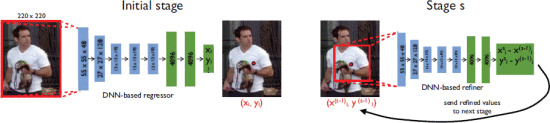
\includegraphics[width=\textwidth]{./images/DeepPose}
	\caption{Архитектура сети DeepPose. \cite{DeepPose}}
	\label{fig:dp_architecture}
\end{figure}



\subsubsection{AlphaPose}
\label{subsubsec:alphapose_desc}

AlphaPose является основной наработкой проекта Machine Vision and Intelligence Group из Шанхайского университета транспорта (Shanghai Jiao Tong University или SJTU). Это первая модель, которая получила значение метрики mAP на датасете COCO выше 70 (0.7) и выше 80 на MPII. Поддерживается как на Linux, так и на Windows. Обрабатывает видео и поддерживает слежение за человеком в реальном времени через восстановление его скелета.

Исследователи не против объединяться с другими проектами для улучшения качества модели и проработки новый фичей. Одной из таких коопераций стала топология Halpe (см. \autoref{subsec:Theory of keypoint detection}), на основании которой и производится оценка позы человека. Доступными являются варианты также с 17 точками от COCO и 25 и 135 точек от Halpe.

В работе Alpha использует top-down подход. Первым этапом идет Faster R-CNN для детектирования человека и выдачи прямоугольников. После используется модель RMPE для предсказания различных поз, которые может принимать  человек. Последним этапом идет работа p-Pose NMS для устранению избыточных предсказаний. На выходе получается изображение с восстановленными позами людей. Все шаги представлены на \autoref{fig:ap_structure}. \cite{fang2017rmpe}

\begin{figure}[h]
	\centering
	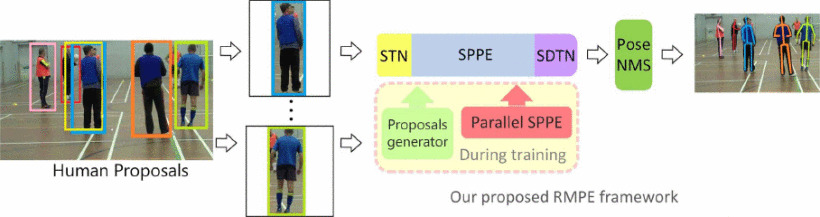
\includegraphics[width=\textwidth]{./images/AlphaPose_structure}
	\caption{Пример работы сети AlphaPose. \cite{fang2017rmpe}}
	\label{fig:ap_structure}
\end{figure}

Рассмотрим поближе модель предсказания. Она использует симметричное преобразование spatial transformer network (STN) и обратное ему spatial de-transformer network (SDTN). Они введены для исправления ошибок локализации, так как SPPE, представленная между ними (см. \autoref{fig:ap_architecture}), является очень чувствительной к неточностям прямоугольника. При обучении параллельно основной модели добавляется ещё одна SPPE (см. \autoref{fig:ap_architecture}) для корректировки преобразования STN. Таким образом получится приблизить данные, получаемые предсказателем, к идеальным и получить наиболее точный результат.

\begin{figure}[h]
	\centering
	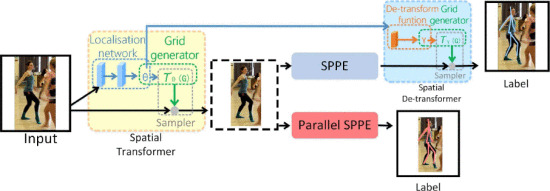
\includegraphics[width=\textwidth]{./images/AlphaPose_architecture}
	\caption{Архитектура сети RMPE. \cite{fang2017rmpe}}
	\label{fig:ap_architecture}
\end{figure}



\subsubsection{BlazePose}
\label{subsubsec:blazepose_desc}

MediaPipe является одним из проектов компании GOOGLE и в своей работе решает задачи компьютерного зрения. В нем уже были представлены модели для распознавания лица (Face Detection) и его поверхности (Face Mesh), ладоней (Hands), объектов (Object Detection и Objectron) и другие \cite{mediapipe}. Для нас же интересна задача поиска ключевых точек, которую и решает модель BlazePose \cite{BlazePose}. На момент исследования модель умеет отслеживать движения человека на видеофрагменте и строить покадровую маску человека.

Для предложенной модели была создана топология, которая представляет собой суперпозицию топологии COCO и двух других топологий, уже использовавшихся в других подпроектах MediaPipe. Об этом более подробно написано в \autoref{subsec:Theory of keypoint detection}.

В BlazePose используется top-down подход оценки позы человека. Сначала запускается Pose Detector (см \autoref{fig:mp_model_structure}), который возвращает координаты интересующей нас области (region-of-interest или ROI). Алгоритм используем расширение модели BlazeFace для определения наличия человека в кадре. Поэтому данная модель чувствительна к видимости головы, лица в частности, на фотографии. Взяв идею витрувианского человека Леонардо Да Винчи, исследователям понадобилось ещё две точки для точной локализации человека на изображении.

\begin{figure}[h]
	\centering
	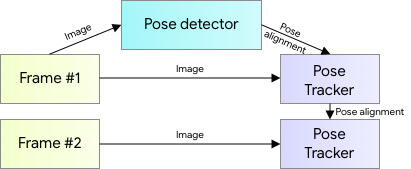
\includegraphics[width=\textwidth * 4 / 5]{./images/MPPose/Model_structure.jpg}
	\caption{Структура модели BlazePose для работы в реальном времени. \cite{BlazePose}}
	\label{fig:mp_model_structure}
\end{figure}

Следующим шагом Pose Tracker производит локализацию каждой точки в заданной ROI. Данное действие производится путем комбинированной обработки тепловой карты и данных о смещении с использованием регрессионной модели (см \autoref{fig:mp_architecture}).

\begin{figure}[h]
	\centering
	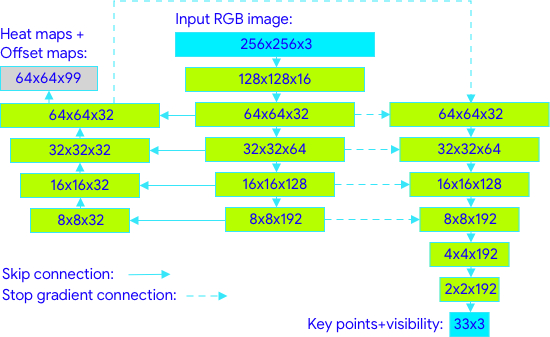
\includegraphics[width=\textwidth * 4 / 5]{./images/MPPose/architecture.jpg}
	\caption{Архитектура модели Pose Tracker. \cite{BlazePose}}
	\label{fig:mp_architecture}
\end{figure}

Как можно заметить из \autoref{fig:mp_model_structure}, при аналитике видеофрагмента Pose Detector используется только на первом кадре, ведь позже данные об интересующей нас области передаются от кадра к кадру. Это упрощает вычисления и позволяет ускорить работу модели в реальном времени.

Развитием данной модели есть ее полное объединение с моделями BlazeFace и BlazeHand в модель Holistic \cite{Holistic}. Она рассматривает намного большее количество точек на лице и ладонях.



\subsubsection{MoveNet.SinglePose}
\label{subsubsec:movenet_desc}

SinglePose создана для работы в веб-интерфейсах или на мобильных устройствах в режиме реального времени. \cite{MoveNet} Модель представлена в двух спецификациях: lightning и thunder. Первая является менее требовательной в плане мощностей и вычислений и способна обрабатывать до 50 кадров в секунду. В то же время, по заверениям создателей, вторая модель имеет большие запросы по ресурсам, но дает лучшую точность распознавания, правда со скоростью до 30 кадров в секунду. 

За расположение ключевых точек выбрана классическая топология COCO. Поэтому модель возвращает координаты 17 точек, которые нормированы на размер изображения (лежат в отрезке [0, 1]).

Представленная модель является восходящей, то есть использует bottom-up подход к решению задачи. Она реализована на архитектуре MobileNetV2 \cite{mobilenetv2} с Feature Pyramid Networks \cite{feature_piramid}, которая используется для извлечения признаков. Обработка результатов магистральной части сети происходит с помощью прогнозирующих головок (см. \autoref{fig:mn_architecture}), которые используют CenterNet \cite{CenterNet} с изменениями, которые повышают быстродействие модели.

\begin{figure}[t]
	\centering
	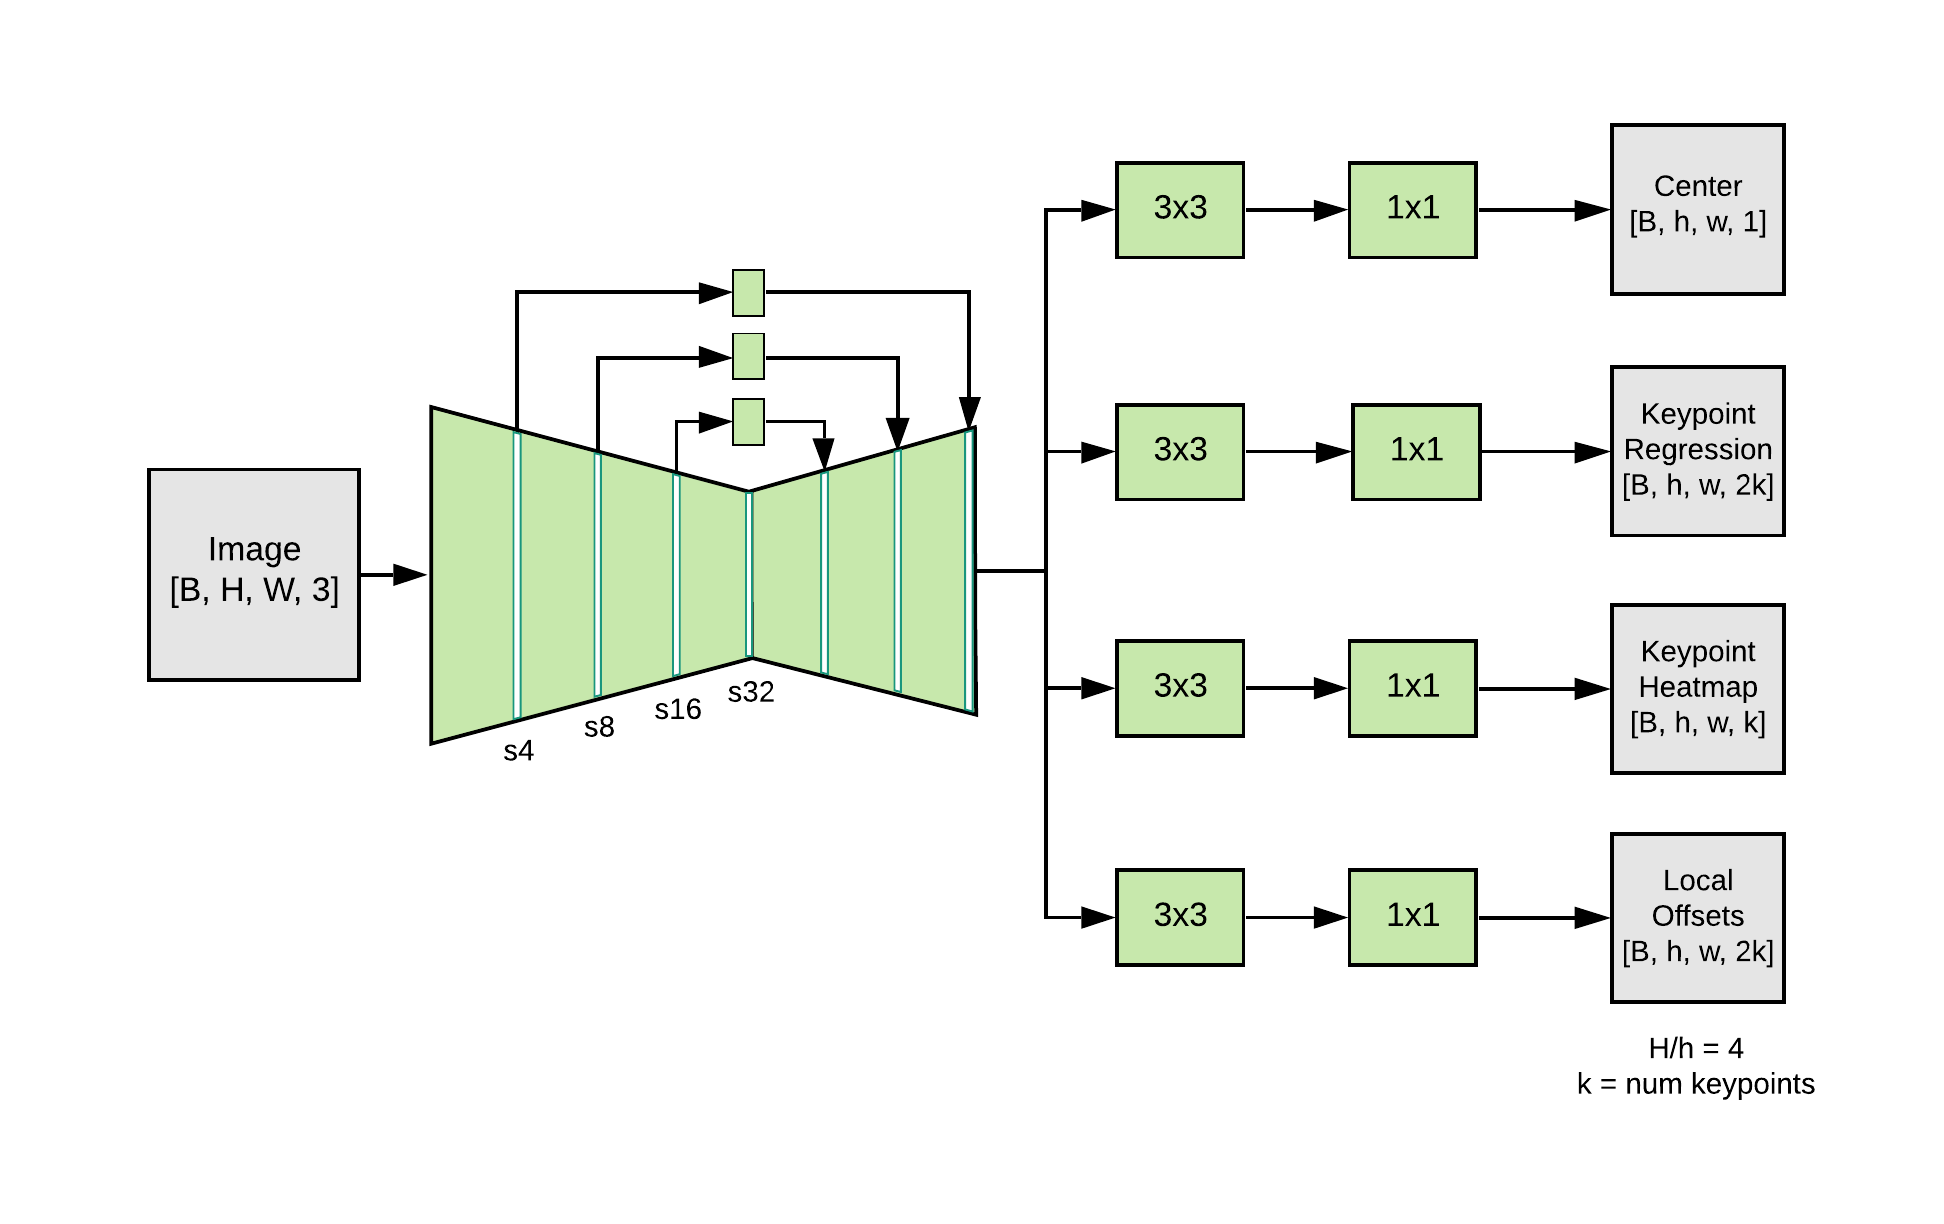
\includegraphics[width=\textwidth * 4 / 5]{./images/MoveNet/architecture}
	\caption{Архитектура модели MoveNet. \cite{MoveNet}}
	\label{fig:mn_architecture}
\end{figure}

Как можно заметить на \autoref{fig:mn_architecture}, 4 прогнозирующие головки отвечают за прогноз карты центральной точки человека, поле регрессионных векторов ключевых точек, карту предсказанных положений ключевых точек и поле смещения ключевых точек. Результаты каждого предсказания вырабатываются параллельно и далее путем последовательной обработки (см. \autoref{fig:mn_structure}) уточняются координаты каждой ключевой точки.

\begin{figure}[h]
	\centering
	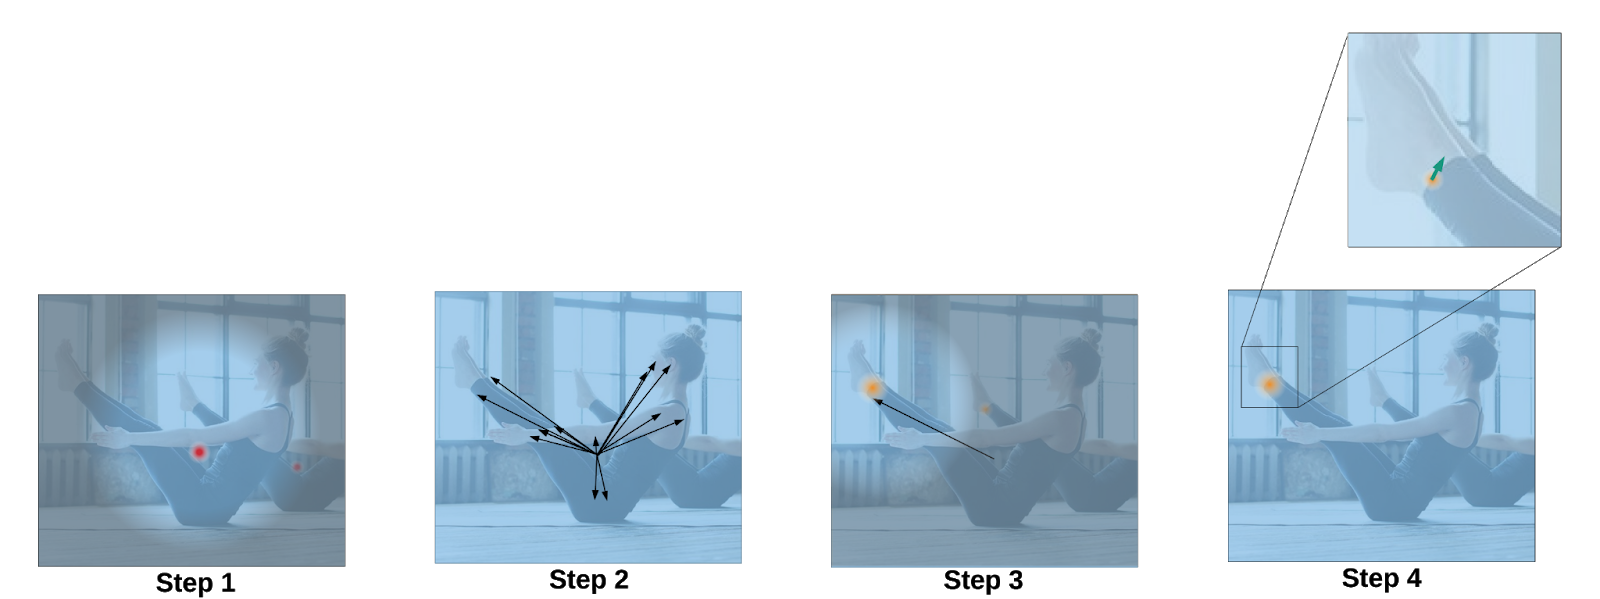
\includegraphics[width=\textwidth * 4 / 5]{./images/MoveNet/structure}
	\caption{Шаги работы prediction head в MoveNet. \cite{MoveNet}}
	\label{fig:mn_structure}
\end{figure}

Такая система позволяет получать точные результаты оценки позы в реальном времени и настроена на обработку в реальном времени изображений, поступающих с камер устройств пользователя.

Следующим этапом развития проекта стала модель MoveNet.MultiPose для распознавания сразу нескольких людей на изображении. Разработчики не стали изменять традициям и представили ее также в двух вариантах: lightning и thunder. А также она использует ту же MobileNetV2 в основе своей работы.



\subsubsection{OpenPose}
\label{subsubsec:openpose_desc}

OpenPose (OP) - это подпроект CMU-Perceptual-Computing-Lab из университета Карнеги-Меллона. В нем представлены различные модели: от локализации точного положения кистей и лица, до определения позы, исследуя 135 точек на теле человека. Также ОР может распознавать нескольких человек одновременно и поддерживает отслеживание скелета человека на видеозаписи в реальном времени через веб-камеру.

В текущей работе рассмотрим модель, работающую по топологии из 25 точек - чем-то похожую на топологию Halpe (см. \autoref{subsec:Theory of keypoint detection}). Особенностью является определение положения стоп за счет детекции 3 дополнительных точек на каждой из них.

OpenPose тоже использует сверточные нейронные сети для решении задачи распознавания ключевых точек с помощью bottom-up подхода. В своей работе исследователи используют понятия карты достоверности обнаружения точки, карты двумерных векторных полей ориентации конечностей (Part Affinity Fields или PAFs) и графы соответствия обнаруженных точек определенным людям на изображении.

Первым шагом происходит обработка изображения и построение карт достоверности и PAFs, про которое поговорим позже. Вторым шагов происходит сопоставление точек и конечностей отдельным людям с использованием графов соответствия. Они помогают решить данную задачу и быстрее решать задачу построения скелетов нескольких человек. В итоге на выходе имеются скелеты нескольких человек. Все шаги представлены на \autoref{fig:op_structure}.

\begin{figure}[h]
	\centering
	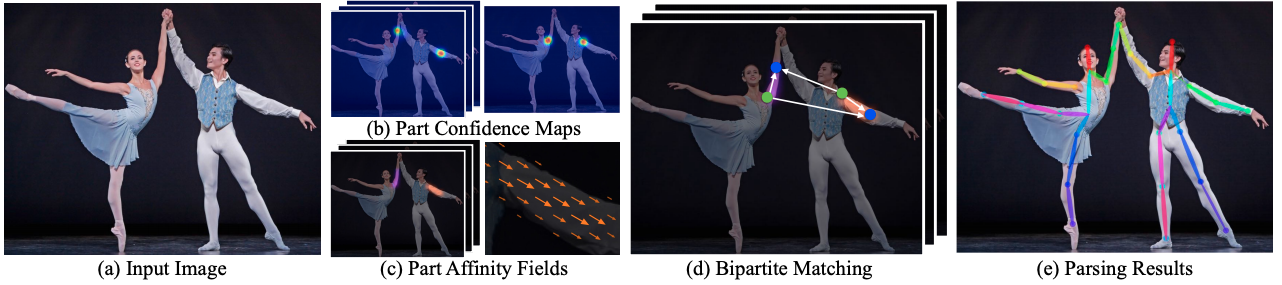
\includegraphics[width=\textwidth]{./images/OpenPose/structure}
	\caption{Последовательность распознавания ключевых точек моделью OpenPose. \cite{OpenPose}}
	\label{fig:op_structure}
\end{figure}

В первоначальной версии модели \cite{OpenPose_first} вычисление карт достоверности и PAFs происходило параллельно, в два этапа. Но в последней работе \cite{OpenPose} предсказания поставили последовательно, так как из PAFs интуитивно можно предсказать и уточнить карты достоверности обнаружения точки (см. \autoref{fig:op_architecture}). Ещё были заменены ядра свертки размером 7х7 на блоки из 3-х последовательных ядер 3х3 (см. \autoref{fig:op_architecture}). Эти преобразование помогло почти в 200 раз увеличить скорость распознавания и в 7 раз улучшить точность.

\begin{figure}[h]
	\centering
	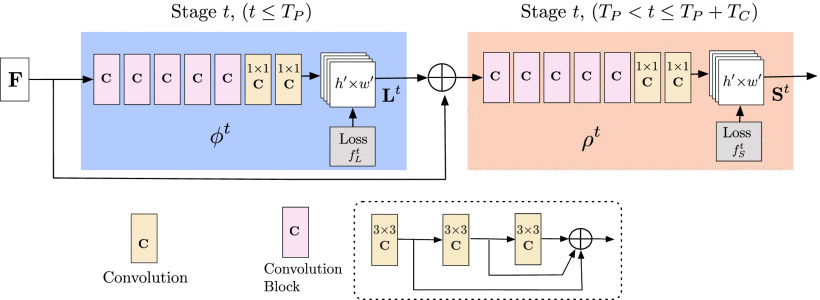
\includegraphics[width=\textwidth * 4 / 5]{./images/OpenPose/architecture.jpg}
	\caption{Архитектура модели OpenPose 2D Pose Estimation. \cite{OpenPose}}
	\label{fig:op_architecture}
\end{figure}



\subsubsection{MMPose}
\label{subsubsec:mmpose_desc}

MMPose - является подпроектом лаборатории Open-MMLab \cite{mmpose2020}. Первым проектом лаборатории было решение задачи детектирования объектов, но позже развивались и другие связанные с компьютерным зрением. Изначально было исследование классификации движений с помощью сетей ST-GCN \cite{STGCN}, но оценку позы решили вынести в отдельную работу. Так появился проект MMPose, включающий в себя распознавание ключевых точек и восстановление скелета человека, модель Animal для тех же задач, но на теле животных. Причем задачи, связанные с человеком, имеют решения с получением предсказаний в 2-х мерном и в 3-х мерном вариантах.

Данная модель постоянно улучшается и подключает новые мировые достижения в свои работы. MMPose использует top-down подход в своей работе и другие наработки лаборатории Open-MMLab. Для работы необходимо сначала использовать detection model, а потом уже передать данные о локализованных людях в pose model.

Детектор натренирован на датасете COCO и выдает предсказания в соответствии с его 17 точечной топологией. Также есть скрипты для обучения на других наборах данных, за что спасибо разработчикам. Правда эти наборы данных надо сначала скачать, но об этом в \autoref{sec:Chapter4}.
\hfill \break






\subsection{Модели для классификации позы человека}
\label{subsec:pose_classification_models}

Далее будет представлено рассмотрение 3 различных модели, которые можно использовать для классификации движений человека.



\subsubsection{Классификатор от MediaPipe}
\label{subsubsec:mp_classificator_desc}

Проект представил модель для оценки позы человека (см. \autoref{subsubsec:blazepose_desc}) и, добавив к нему k-NN, получили алгоритм классификации позы человека. Таким образом MediaPipe представило программу для счета приседаний или отжиманий с камеры смартфона в реальном времени. \cite{mediapipe_cls}

Для работы использовалась топология BlazePose, а точнее вектор расстояний между некоторыми точками этой топологии (см. \autoref{fig:blazepose_classificator}). Так как в реальных изображениях бывают разные масштабы и размеры, то все позы нормализуются и переориентируются в вертикальное положение.

\begin{figure}[h]
	\centering
	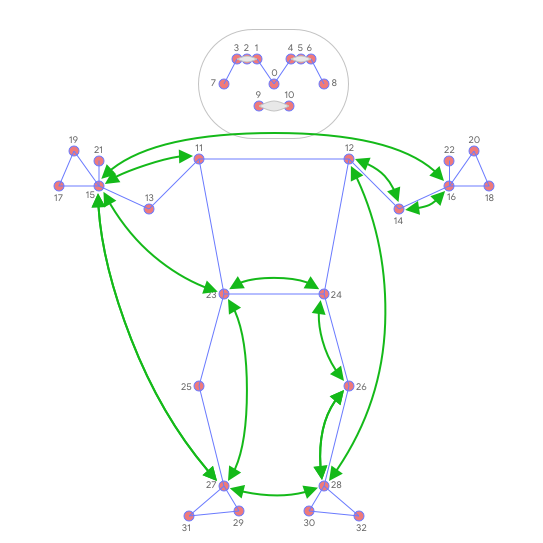
\includegraphics[width=0.6\textwidth]{./images/Classificators/BlazePose}
	\caption{Расстояния между точками топологии BlazePose, которые используются в классификации. \cite{mediapipe_cls}}
	\label{fig:blazepose_classificator}
\end{figure}

Для обеспечения точности классификации разработчики решили запускать k-NN дважды: первый раз для отбора векторов признаков для похожих с целевой поз, а во второй раз для отбора точной позы среди выбранных ранее. Различия в том, что используются различные метрики минимальное покоординатное расстояние и среднее покоординатное расстояния для первого и второго прогона соответственно.



\subsubsection{mmakos}
\label{subsubsec:mmakos_desc}

Модель является бакалаврской работой студента Варшавского университета Михала Макоса \cite{mmakos}. Классификатор работает с видеоданными и разделяет модели на два супер класса: статические и динамические.

Разработчик взял за основу модель распознавания позы человека OpenPose (см. \autoref{subsubsec:openpose_desc}) и преобразовал входные данные из 4-х мерного формата в 2-мерное изображение (см. \autoref{fig:mmakos_image_prep}). По сути три координаты каждой ключевой точки преобразовывались в BGR формат и создавался столбец пикселей для текущего момента времени. При рассмотрении 15 точек и 32 кадров получаются переходные изображения размером (15, 32, 3).

\begin{figure}[h]
	\centering
	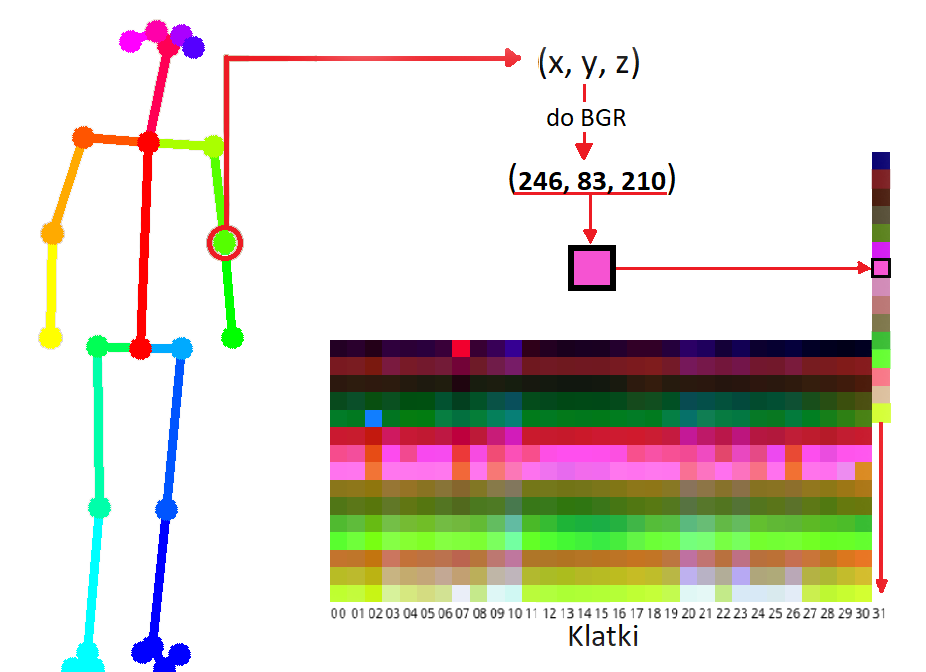
\includegraphics[width=0.6\textwidth]{./images/Classificators/MMakos_image_prep}
	\caption{Преобразование данных в модели от M. Makos. \cite{mmakos}}
	\label{fig:mmakos_image_prep}
\end{figure}
\hspace{1cm}

Для классификации используется версия сети VGG. По решению автора все позы делятся на два супер-класса: динамические и статические, а потом уже классифицируются внутри супер-классов более точно.



\subsubsection{MMaction2 by OpenMMlab}
\label{subsubsec:mmaction2_desc}

MMAction2 является подпроектом лаборатории Open-MMLab \cite{2020mmaction2}. Идея классификации движения начиналась с проекта MMSkeleton построенном на исследовании про ST-GCN \cite{STGCN} и позже переросло в первую версию MMAction для классификации движений одного человека. Текущая версия может обрабатывать взаимоотношения между людьми, такие как обнимания или рукопожатия. 

Для классификации необходимо сначала обработать видеофрагмент. Для этого производится поиск и локализация действия во времени, а также восстановление и анализ скелета.

В первом случае используется TimeSformer \cite{TimeSformer} - создан на основе идеи Transformer для обработки видеопотоков. Он использует несколько видов блоков Attention (см. \autoref{fig:timesformer}) для объединения информации на нескольких кадрах до и после текущего. Это дает возможность точно распознавать действия в кадре и отслеживать их.

\begin{figure}[h]
	\centering
	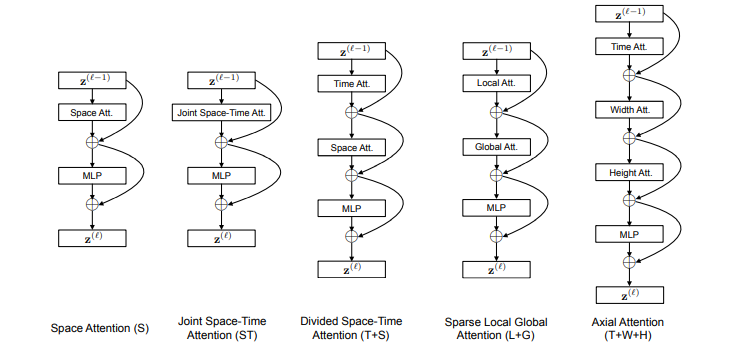
\includegraphics[width=0.9\textwidth]{./images/Classificators/TimeSformer}
	\caption{Примеры блоков внимания в TimeSformer. \cite{TimeSformer}}
	\label{fig:timesformer}
\end{figure}

Для обработки скелетов используется модель PoseC3D \cite{duan2021revisiting}. Она использует несколько тепловых 3D-карт в качестве представления скелета человека и за счет этого обходит GCN и более устойчив к шумам на изображении. Также без особенно лишних затрат можно использовать PoseC3D для классификации взаимодействия между людьми.

\begin{figure}[h]
	\centering
	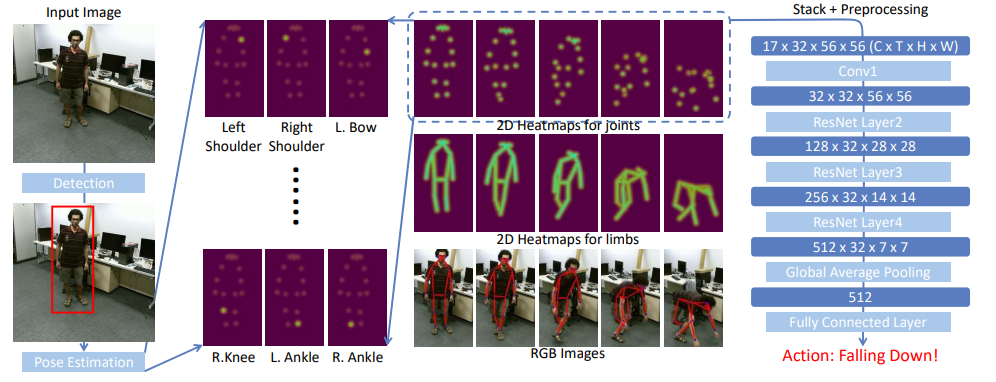
\includegraphics[width=\textwidth]{./images/Classificators/PoseC3D}
	\caption{Структура сети PoseC3D. \cite{duan2021revisiting}}
	\label{fig:posec3d}
\end{figure}

Все исследования проекта основаны на классификации и анализе видео, что полезно для будущих исследований и развитии темы работы.


\newpage %% Обзор существующих решений
    \section{Поиск данных}
\label{sec:Chapter3} \index{Chapter3}
Здесь надо декомпозировать большую задачу из постановки на подзадачи и продолжать этот процесс, пока подзадачи не станут достаточно простыми, чтобы их можно было бы решить напрямую (например, поставив какой-то эксперимент или доказав теорему) или найти готовое решение.

\subsection{Data for Pose Estimation}

\subsubsection{LSP}

\subsubsection{MPII HRD}

\subsubsection{COCO keipoints}

\subsection{Data for Pose Classification}

\subsubsection{HPC/mmakos}

\subsubsection{MPII}

\subsubsection{Yoga-82}

\subsection{Not Available data}

\subsubsection{Human3.6M}

\subsubsection{Surreal}

\subsubsection{BUFF}

\newpage %% Поиск данных
    \section{Исследование моделей}
\label{sec:Chapter4} \index{Chapter4}

В данной главе будет представлено описание и результаты исследования моделей: BlazePose, MoveNet.SinglePose, OpenPose и MMPose.


\subsection{Описание эксперимента}

Эксперимент включает рассмотрение только моделей распознавания ключевых точек на теле человека, так как это является основной частью решения задачи классификации движений и многие классификаторы движений строятся на выходных данных о позе.

Из представленных в \autoref{subsec:pose_estimation_models} моделей были выбраны 4 представителя по некоторым критериям:

\begin{itemize}
	\item Доступность модели для исследований\\
	Необходимо оценить длительность установки и возможности работы с различными операционными системами. Эксперимент проводился на платформе Google Colab, поэтому необходимо было рассмотреть возможность использования модели на в Colaboratory.
	\item Новизна модели\\
	Представленная выборка была создана в основном в 2010-х, но модель DeepPose является самой старой. Новые разработки опирались на результаты, полученные в ней, и таким образом получали более хорошие результаты.
	\item Наличие документации\\
	Все модели производят классификацию по двум осям изображения: высота и ширина, а также по параметру видимость ключевой точки. Некоторые модели выдают данные нормированные на размер изображения (число из отрезка [0,1]), а некоторые точное значение в пикселях. Поэтому для работы необходимо было понимать как работает API модели, какие у нее входные - выходные данные.
	\item Тренировка модели на датасете COCO\\
	Все используемые претренированные модели были обучены на наборе данных COCO \cite{COCO_topology} в совместительстве с каким-либо другим датасетом. В некоторых  примерах не было возможности использовать претренированную модель и из-за этого они были отсеяны.
\end{itemize}

В итоге было выбрано 4 модели наиболее подходящие под критерии:
\begin{enumerate}
	\item BlazePose
	\item MoveNet.SinglePose
	\item OpenPose
	\item MMpose
\end{enumerate}

Для проведения качественного анализа и выявления лучшей модели необходимо их сравнить. Поэтому рассмотрим метрики, которые подходят для задач в 2-х мерном пространстве:

\begin{itemize}
	\item Percentage of Detection Joints\\
	PDJ оценивает точность распознавания ключевой точки в зависимости от диагональных размеров человека. При рассмотрении задачи распознавания человека на выходе имеются координаты точек, которые характеризуют прямоугольник, внутри которого вписан человек. Диагональ этого прямоугольника используется при высчитывании метрики PDJ (см. \autoref{fig:PDJ}). Формулу можно представить в следующем виде:
	\begin{equation}
		PDJ = \frac{\sum_{i=1}^{n} bool(d_i < threshold * diag)}{n},
	\end{equation}
	
	где\\
	$d_i$ - расстояние между предсказанной и правильной точкой,\\
	$threshold$ - порог, задаваемый исследователем,\\
	$diag$ - размер диагонали прямоугольника, внутри которого находится человек,\\
	$bool()$ - логическое условие, возвращает 1, если оно верно и 0 в ином случае,\\
	$n$ - размер выборки.
	
	С помощью значения порога можно варьировать допустимую погрешность расстояния между истинной и предсказанной точками.
	\begin{figure}[h]
		\centering
		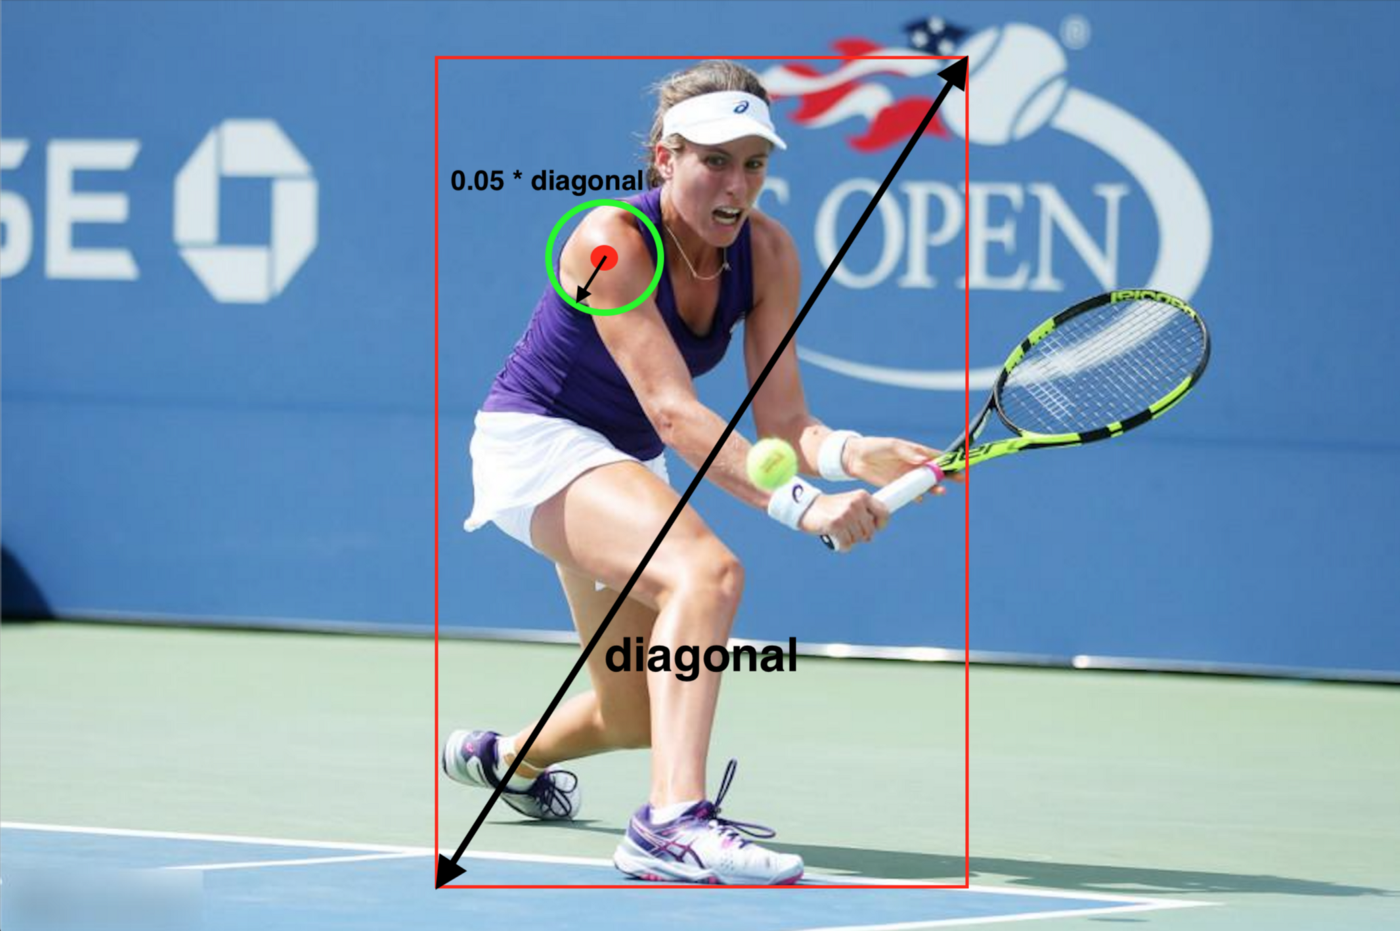
\includegraphics[width=\textwidth * 4 / 5]{./images/PDJ}
		\caption{Визуальное представление метрики PDJ.\\ Зеленый круг ограничивает область допустимого расположения распознанной ключевой точки.}
		\label{fig:PDJ}
	\end{figure}

	\item Percentage of Correct Key-points\\
	PCK очень похожа на предыдущую метрику, только погрешность рассматривается относительно высоты человека. Формулу можно представить в следующем виде:
	\begin{equation}
		PDJ = \frac{\sum_{i=1}^{n} bool(d_i < threshold * body_height)}{n},
	\end{equation}
	
	где\\
	$d_i$ - расстояние между предсказанной и правильной точкой,\\
	$threshold$ - порог, задаваемый исследователем,\\
	$body_height$ - высота прямоугольника, внутри которого находится человек,\\
	$bool()$ - логическое условие, возвращает 1, если оно верно и 0 в ином случае,\\
	$n$ - размер выборки.
	
	\item Object Key-point Similarity\\
	OKS является основной при оценке задачи Keypoint Detection COCO \cite{COCO_topology}. Она использует третью координату выходного предсказания и расстояние между реальной и предсказанной точками. Формулу можно представить в следующем виде:
	\begin{equation}
		OKS = \frac{\sum_{i} exp\left( - d_i^2 / 2s^2k_i^2\right)\delta\left(v_i > 0\right)}{\sum_{i} \delta\left(v_i > 0\right)},
	\end{equation}
	где\\
	$d_i$ - расстояние между предсказанной и правильной точкой,\\
	$s$ - площадь объекта,\\
	$k_i$ - константа ключевой точки, контролирующаю спад,\\
	$v_i$ - видимость.
	
	При оценке задачи детекции ключевых точек COCO вводится метрика Average Precision (AP) через OKS. Изменяя границу допустимого значения OKS можно получать различные значения precision и AP.
\end{itemize}

В метриках PCK и PDJ необходимо знать размеры прямоугольника, ограничивающего человека. Для этого необходимо использовать модель распознавания объектов, которая будет давать нам эти данные. При работе с метрикой PCK можно обойтись без такой модели, потому что во всех топологиях есть точки, которые обозначают верхнюю и нижнюю границы человека. Отсюда погрешность вычисления через модель и вычисления разности ординат верхней и нижней точек будет мала. Что требует меньше затрат для оценки.

\subsection{Поиск данных}

Первым делом необходимо было проверить модели на неразмеченных данных. Для этого были выбраны фотографии высокого разрешения, где человек изображен во весь рост (см. \autoref{fig:test_photos}).

\begin{figure}[h]
\begin{subfigure}[b]{.5\textwidth}
	\centering
	
\includegraphics[width=\textwidth]{./images/Test/ролики2}
	\caption{ }
\end{subfigure}
\begin{subfigure}[b]{.5\textwidth}
	\centering
  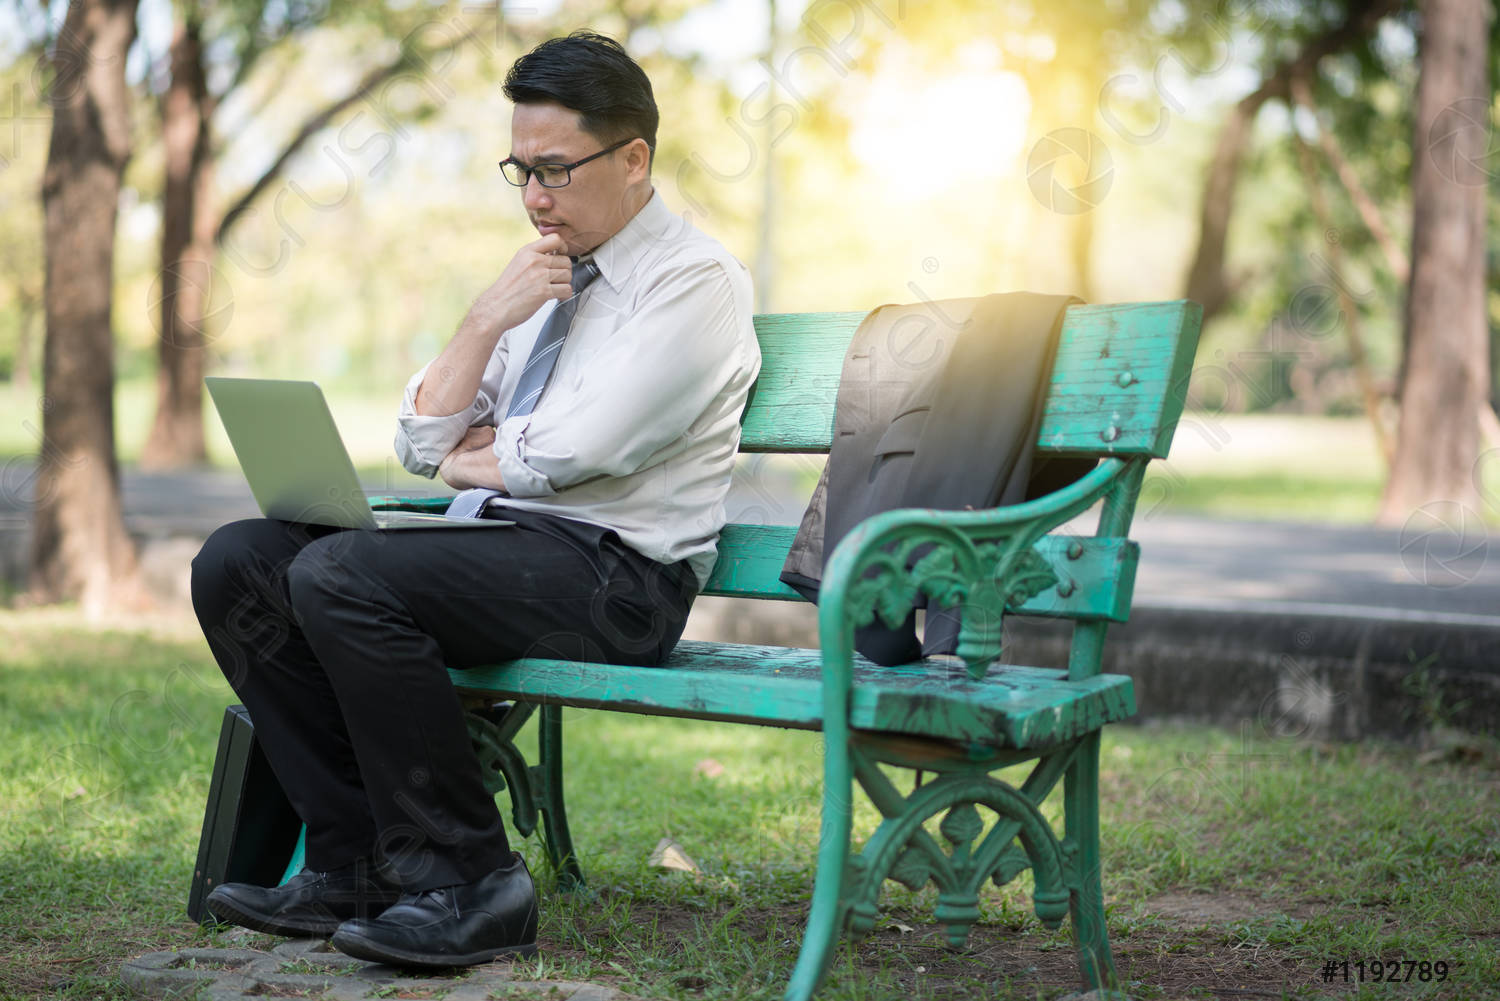
\includegraphics[width=\textwidth]{./images/Test/скамека3}
  \caption{ }
\end{subfigure}
\begin{subfigure}[b]{.5\textwidth}
	\centering
  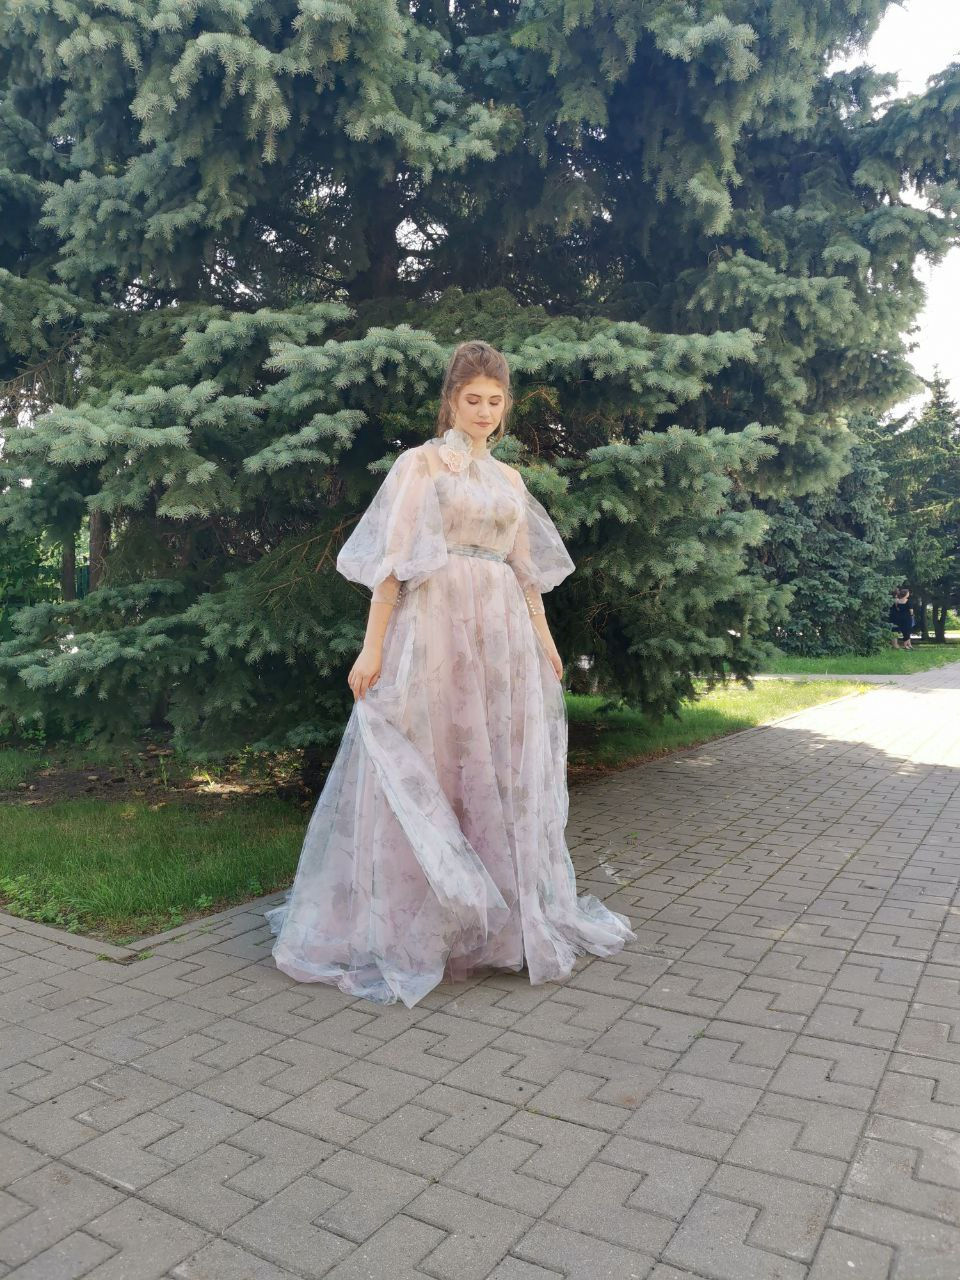
\includegraphics[height=\textwidth]{./images/Test/dress}
  \caption{ }
\end{subfigure}
\begin{subfigure}[b]{.5\textwidth}
	\centering
  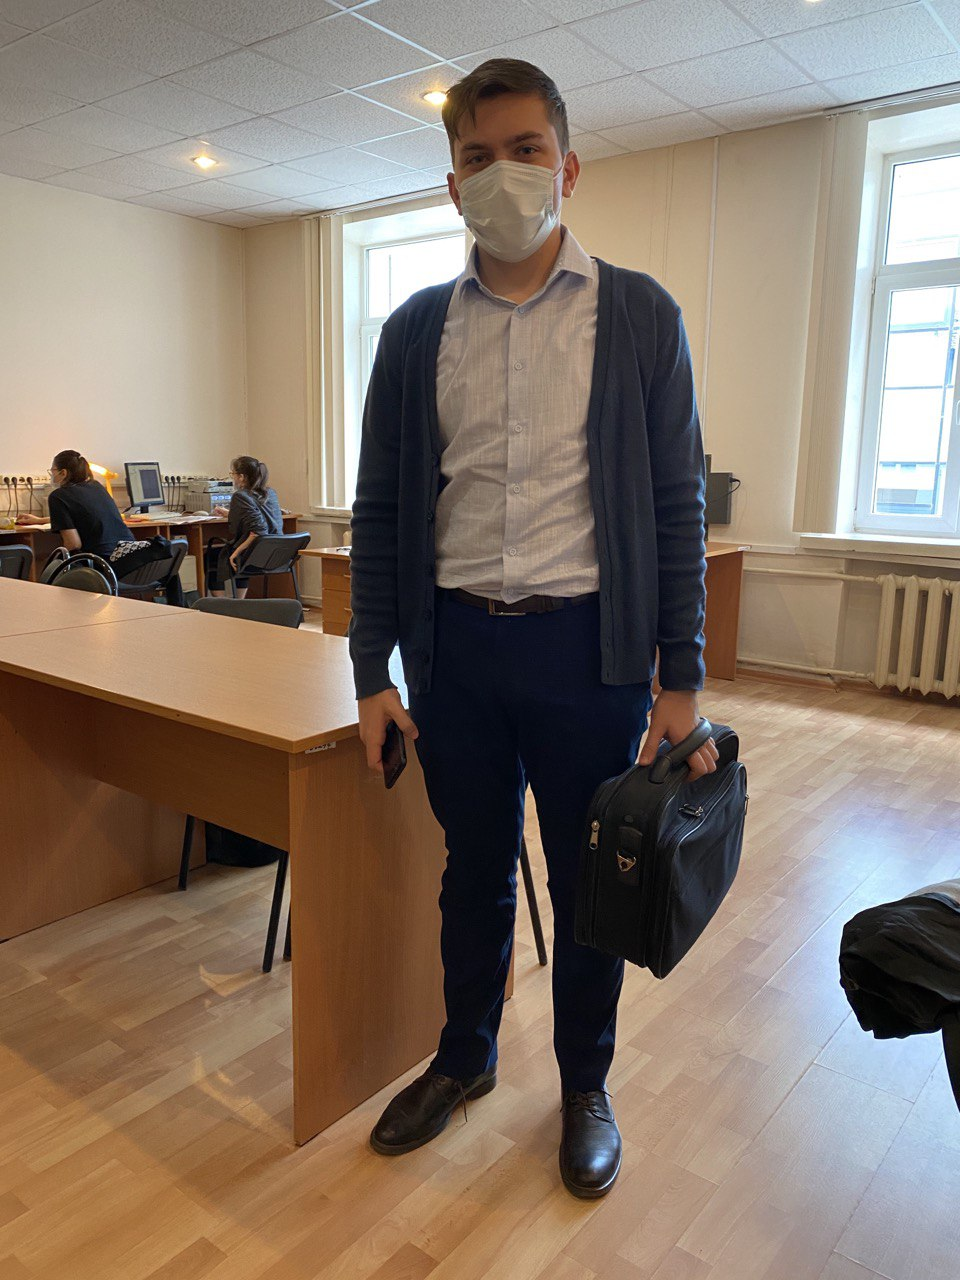
\includegraphics[height=\textwidth]{./images/Test/static}
  \caption{ }
\end{subfigure}
  \caption{Изображения для визуальной оценки моделей.}
  \label{fig:test_photos}
\end{figure}

Для качественной оценки работы моделей с помощью метрик необходимо было найти размеченные данные. Приведу описание датасетов, которые были мной рассмотрены:

\begin{itemize}
	\item COCO Dataset и MPII\\
	Данные наборы являются основными при работе с компьютерным зрением и большинство исследователей используют их как тренировочные для своих моделей. Поэтому использовать их в качестве тестовых не целесообразно. \cite{COCO_dataset, MPII_dataset}
	\item HUMAN 3.6M\\
	Данные собирались специально для задачи классификации движений человека в студии. С помощью датчиков фиксировались положения всех суставов и ключевых точек. Это идеальный датасет, но доступ к нему ограничен и создатель не выходит на связь. \cite{h36m_pami}
	\hfill \break
	\item LSP\\
	Данные собраны со спортивных соревнований и пред обработаны до обозначения одного человека на изображении размером не менее 150 пикселей в высоту. Единственная проблема - не описаны точки на лице, поэтому оценивать можно только распознавание 12 суставов или, другими словами, точек на теле человека. \cite{LSP}
	\item LSP Extended\\
	Является расширенной версией предыдущего набора данных. По объёму превосходит его в пять раз. Остальные характеристики не поменялись. \cite{LSPE}
	\item Halpe\\
	Датасет для распознавания точек на всем теле человека. К каждой фотографии идет аннотация из 136 точек, краев ограничивающего прямоугольника и категории детектируемого объекта (во всех фотографиях стоит категория человек).
	
	Набор состоит из двух частей: HICO-DET и COCO. Все они аннотированны описанные выше способом. Для наших моделей необходимо будет отобрать только 17 точек, совпадающих с топологией СОСО. \cite{Halpe_dataset}
\end{itemize}

Выше были представлены наборы данных для задачи распознавания точек на теле человека. Но основной темой является классификация движений человека, поэтому необходимы фотографии с меткой класса для позы, представленной на данных. Некоторые из уже представленных (COCO, MPII) тоже могут использоваться для классификации позы, но по тем же причинам, что и описаны выше, они не будут рассмотрены в эксперименте. Приведу описание датасетов для классификации движения человека по позе на изображении:


\begin{itemize}
	\item Stanford-40\\
	Набор данных состоит примерно из 10 тыс. изображений, на каждом из которых человек делает одно из 40 действий. На один класс приходится от 180 до 300 фотографий. \cite{stanford40}
	\item Yoga-82\\
	Сложность распознавания поз йоги в том, что многие из них не могут быть точно аннотированы. Для решения этой проблемы и был собран этот набор данных вмещающий примерно 28 тыс. изображений. 82 различные позы разделены по 6 подклассам. При желании можно использовать метки и классов, и подклассов для классификации. \cite{verma2020yoga}
\end{itemize}

Итого были выбраны наборы данных LSP, LSPE и Halpe. \begin{figure}[h]
\begin{subfigure}[b]{.2\textwidth}
	\centering
	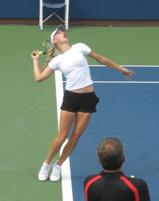
\includegraphics[height=\textwidth]{./images/LSP1}
\end{subfigure}
\begin{subfigure}[b]{.1\textwidth}
	\centering
  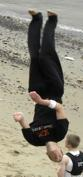
\includegraphics[height=2\textwidth]{./images/LSP2}
\end{subfigure}
\begin{subfigure}[b]{.2\textwidth}
	\centering
  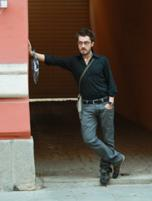
\includegraphics[height=\textwidth]{./images/LSP3}
\end{subfigure}
\begin{subfigure}[b]{.15\textwidth}
	\centering
  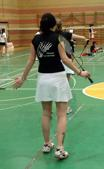
\includegraphics[height=4\textwidth / 3]{./images/LSP4}
\end{subfigure}
\begin{subfigure}[b]{.15\textwidth}
	\centering
  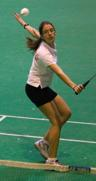
\includegraphics[height=4\textwidth / 3]{./images/LSP5}
\end{subfigure}
\begin{subfigure}[b]{.15\textwidth}
	\centering
  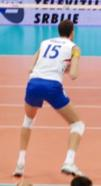
\includegraphics[height=4\textwidth / 3]{./images/LSP6}
\end{subfigure}
  \caption{Примеры изображений из датасета LSP.}
  \label{fig:dataset_photos}
\end{figure}

\subsection{Результаты эксперимента}

Для каждой модели была рассмотрена локализация ключевых точек на фотографиях высокого качества (см. \autoref{fig:test_photos}), а также набор данных низкого качества с обработанными изображениями.

Метрики были рассчитаны с порогами 0.05, 0.2, 0.5. В дополнение к этому был проведен временной анализ классификации одного изображения в среднем по целому датасету.

Перейдем к результатам по каждой модели.
\hfill \break

\textbf{
	\begin{large}
		BlazePose
	\end{large}
}

Результаты работы модели можно посмотреть на \autoref{fig:MP_result}. Как можно заметить, некоторые точки не распознаются и не отображаются на итоговом результате. А также есть небольшая погрешность при распознавании глаз. Но модель хорошо сработала на человека в маске.

Исходя из значений метрик (см. в \autoref{tab:MP_table}) можно сделать вывод, что модель имеет высокую погрешность при среднем времени обработки одной фотографии 0.063 секунды.

\begin{table}[h]
	\centering
	\begin{tabular}{|p{1.5cm}||p{2.2cm}|p{2cm}|p{2cm}|p{2.2cm}|p{2cm}|p{2cm}|}
		\hline
		Metric&PCK@0.05&PCK@0.2&PCK@0.5&PDJ@0.05&PDJ@0.2&PDJ@0.5\\\hline
		\hline
		LSP & 0.035 & 0.304 & 0.741 & 0.042 & 0.359 & 0.815\\
		LSPE & 0.005 & 0.059 & 0.277 & 0.009 & 0.108 & 0.457\\
		Halpe & 0.004 & 0.051 & 0.222 & 0.005 & 0.077 & 0.313\\
		\hline
	\end{tabular}
	\begin{tabular}{|p{1.5cm}||p{2cm}|p{2cm}|p{2cm}|}
		\hline
		Metric&AP@0.5&AP@0.75&AP\\\hline\hline
		LSP & 0.012 & 0.004 & 0.006\\
		LSPЕ & 0.03 & 0.001 & 0.001\\
		\hline
	\end{tabular}
	\caption{Результаты вычисления метрик для BlazePose.}
	\label{tab:MP_table}
\end{table}
\hspace{1cm}

\textbf{
	\begin{large}
		MoveNet.SinglePose
	\end{large}
}

Результаты работы модели можно посмотреть на \autoref{fig:MN_result}. Заметны огрехи в распознавании локтей и ладоней. Как и в прошлой модели есть неточности при распознавании частей лица.

Исходя из значений метрик (см. в \autoref{tab:MN_table}) можно сделать вывод, что модель показала себя плохо при оценивании с порогом 0.05, но лучший результат среди всех для порогах 0.2 и 0.5. Среднее время обработки одной фотографии составило 0.009 секунды, что также является наилучшим показателем.

\begin{table}[h]
	\centering
	\begin{tabular}{|p{1.5cm}||p{2.2cm}|p{2cm}|p{2cm}|p{2.2cm}|p{2cm}|p{2cm}|}
		\hline
		Metric&PCK@0.05&PCK@0.2&PCK@0.5&PDJ@0.05&PDJ@0.2&PDJ@0.5\\\hline
		\hline
		LSP & 0.356 & 0.928 & 0.983 & 0.43 & 0.95 & 0.993\\
		LSPE & 0.144 & 0.539 & 0.745 & 0.227 & 0.635 & 0.806\\
		Halpe & 0.04 & 0.052 & 0.223 & 0.006 & 0.078 & 0.32\\
		\hline
	\end{tabular}
	\begin{tabular}{|p{1.5cm}||p{2cm}|p{2cm}|p{2cm}|}
		\hline
		Metric&AP@0.5&AP@0.75&AP\\\hline\hline
		LSP & 0.168 & 0.064 & 0.08\\
		LSPЕ & 0.312 & 0.059 & 0.111\\
		\hline
	\end{tabular}
	\caption{Результаты вычисления метрик для MoveNet.SinglePose.}
	\label{tab:MN_table}
\end{table}
\hspace{1cm}


\textbf{
	\begin{large}
		OpenPose
	\end{large}
}

Результаты работы модели можно посмотреть на \autoref{fig:OP_result}.

Значения метрик см. в \autoref{tab:OP_table}.

Среднее время обработки одной фотографии составило 0.037 секунды.

Визуально лучший результат обработки изображений, хотя по метрикам немного уступает следующей модели. Но полностью обыгрывает ее во времени обработки.

\begin{table}[h]
	\centering
	\begin{tabular}{|p{1.5cm}||p{2.2cm}|p{2cm}|p{2cm}|p{2.2cm}|p{2cm}|p{2cm}|}
		\hline
		Metric&PCK@0.05&PCK@0.2&PCK@0.5&PDJ@0.05&PDJ@0.2&PDJ@0.5\\\hline
		\hline
		LSP & 0.708 & 0.837 & 0.882 & 0.746 & 0.845 & 0.899\\
		LSPE & 0.362 & 0.524 & 0.633 & 0.42 & 0.569 & 0.69\\
		Halpe & 0.575 & 0.638 & 0.686 & 0.613 & 0.658 & 0.72\\
		\hline
	\end{tabular}
	\begin{tabular}{|p{1.5cm}||p{2cm}|p{2cm}|p{2cm}|}
		\hline
		Metric&AP@0.5&AP@0.75&AP\\\hline\hline
		LSP & 0.166 & 0.085 & 0.092\\
		LSPЕ & 0.538 & 0.362 & 0.362\\
		Halpe & 0.562 & 0.398 & 0.384\\
		\hline
	\end{tabular}
	\caption{Результаты вычисления метрик для OpenPose.}
	\label{tab:OP_table}
\end{table}

\textbf{
	\begin{large}
		MMPose
	\end{large}
}

Результаты работы модели можно посмотреть на \autoref{fig:MMP_result}.

Значения метрик см. в \autoref{tab:MMP_table}.

Среднее время обработки одной фотографии составило 0.409 секунды.

Для своей работы требует детекции человека, из-за чего показывает лучший результат в точности, но худший результат по времени обработки одного изображения.

\begin{table}[h]
	\centering
	\begin{tabular}{|p{1.5cm}||p{2.2cm}|p{2cm}|p{2cm}|p{2.2cm}|p{2cm}|p{2cm}|}
		\hline
		Metric&PCK@0.05&PCK@0.2&PCK@0.5&PDJ@0.05&PDJ@0.2&PDJ@0.5\\\hline
		\hline
		LSP & 0.728 & 0.85 & 0.914 & 0.76 & 0.858 & 0.933\\
		LSPE & 0.403 & 0.56 & 0.651 & 0.463 & 0.587 & 0.72\\
		Halpe &  &  &  &  &  & \\
		\hline
	\end{tabular}
	\begin{tabular}{|p{1.5cm}||p{2cm}|p{2cm}|p{2cm}|}
		\hline
		Metric&AP@0.5&AP@0.75&AP\\\hline\hline
		LSP & 0.225 & 0.223 & 0.123\\
		LSPЕ & 0.598 & 0.462 & 0.443\\
		Halpe &  &  & \\
		\hline
	\end{tabular}
	\caption{Результаты вычисления метрик для MMPose.}
	\label{tab:MMP_table}
\end{table}
\hfill \break

\textbf{
	\begin{large}
		Визуализация результатов
	\end{large}
}

На \autoref{fig:results_pck} и \autoref{fig:results_pdj} представлены средние для трех датасетов (LSP, LSPE и Halpe) метрик PCK и PDJ соответственно. Модель BlazePose является явным аутсайдером. OpenPose и MMPose показывают качественные результаты при любых порогах допустимой погрешности. А MoveNet имеет лучшие результаты при большей ошибке.

Результаты растут с увеличением порога, так как увеличивается и допустимая погрешность локализации. Следовательно и количество верных точек тоже становится больше.

\begin{figure}[h]
	\centering
	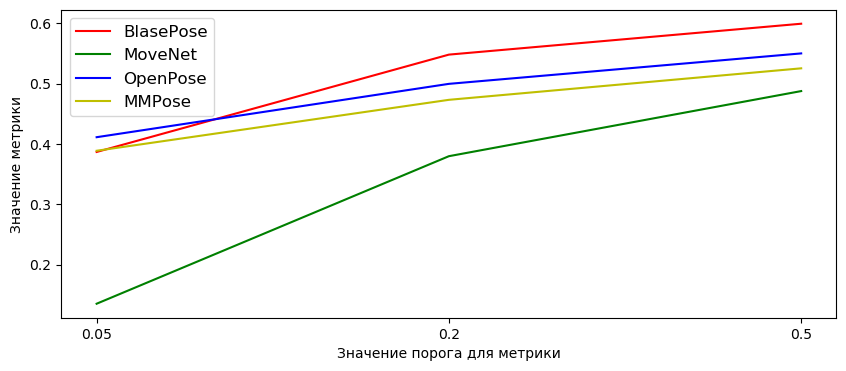
\includegraphics[width=0.97\textwidth]{./images/results/PCK}
	\caption{Средние значения метрики PCK.}
	\label{fig:results_pck}
\end{figure}

\begin{figure}[h]
	\centering
   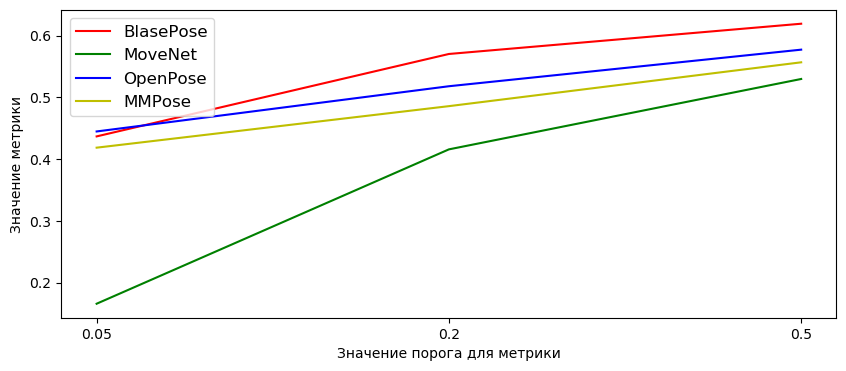
\includegraphics[width=0.97\textwidth]{./images/results/PDJ}
   \caption{Средние значения метрики PDJ.}
   \label{fig:results_pdj}
\end{figure}

На \autoref{fig:results_ap} представлены значения метрики AP также по всем трем наборам данных. Здесь первые две модели (BlazePose и MoveNet) ушли в аутсайдеры из-за плохого результата на изображениях из Halpe, в то время как две другие (OpenPose и MMPose) наоборот выросли за счет этих фотографий.

Результаты данной метрики убывают, так как с увеличением порога метрики растет минимально допустимое значение OKS, которое необходимо для определения верного распознавания.

\begin{figure}[h]
	\centering
   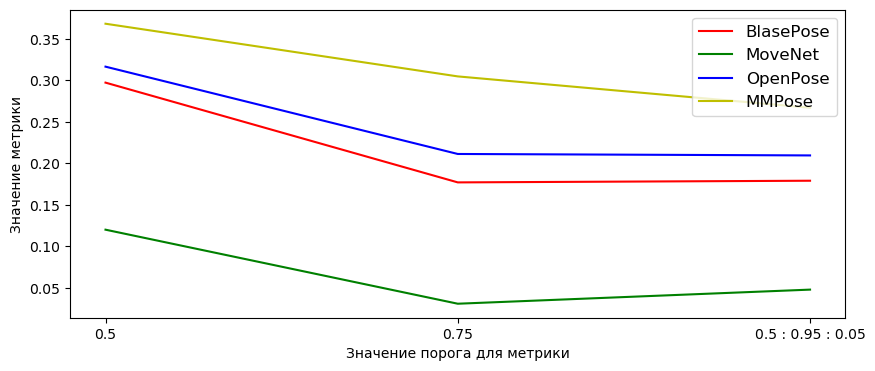
\includegraphics[width=0.97\textwidth]{./images/results/AP}
   \caption{Средние значения метрики AP.}
   \label{fig:results_ap}
\end{figure}


\newpage
 %% Эксперимент
    \section{Заключение}
\label{sec:Chapter5} \index{Chapter5}
Здесь надо перечислить все результаты, полученные в ходе работы. Из текста должно быть понятно, в какой мере решена поставленная задача.

\newpage %% Заключение

    %% Don't change the following lines
    \nocite{*}
    \bibliography{references}

    %% в зависимости от надобности подключаем раздел "Приложениие"
    % \newpage
    % \section{Приложение}
\label{sec:Appendix} \index{Appendix}

\textbf{
	\begin{large}
		Визуальные результаты работы моделей
	\end{large}
}

\begin{figure}[h]
\begin{subfigure}[b]{.5\textwidth}
	\centering
	
\includegraphics[width=\textwidth]{./images/MPPose/19}
	\caption{ }
\end{subfigure}
\begin{subfigure}[b]{.5\textwidth}
	\centering
   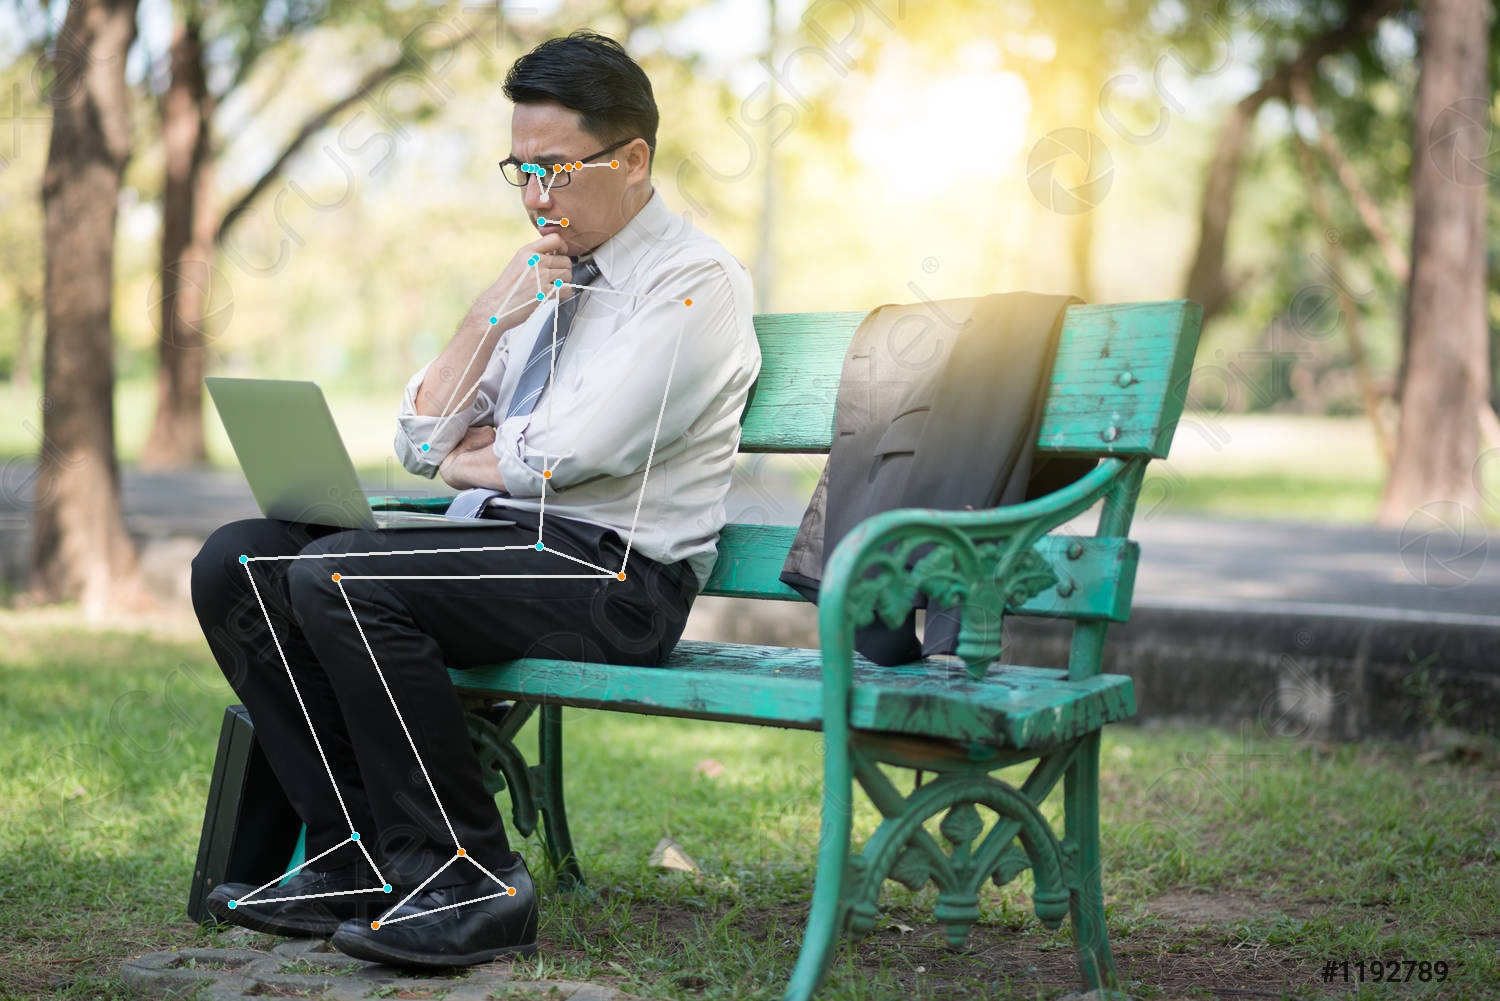
\includegraphics[width=\textwidth]{./images/MPPose/23}
   \caption{ }
\end{subfigure}
\begin{subfigure}[b]{.5\textwidth}
	\centering
   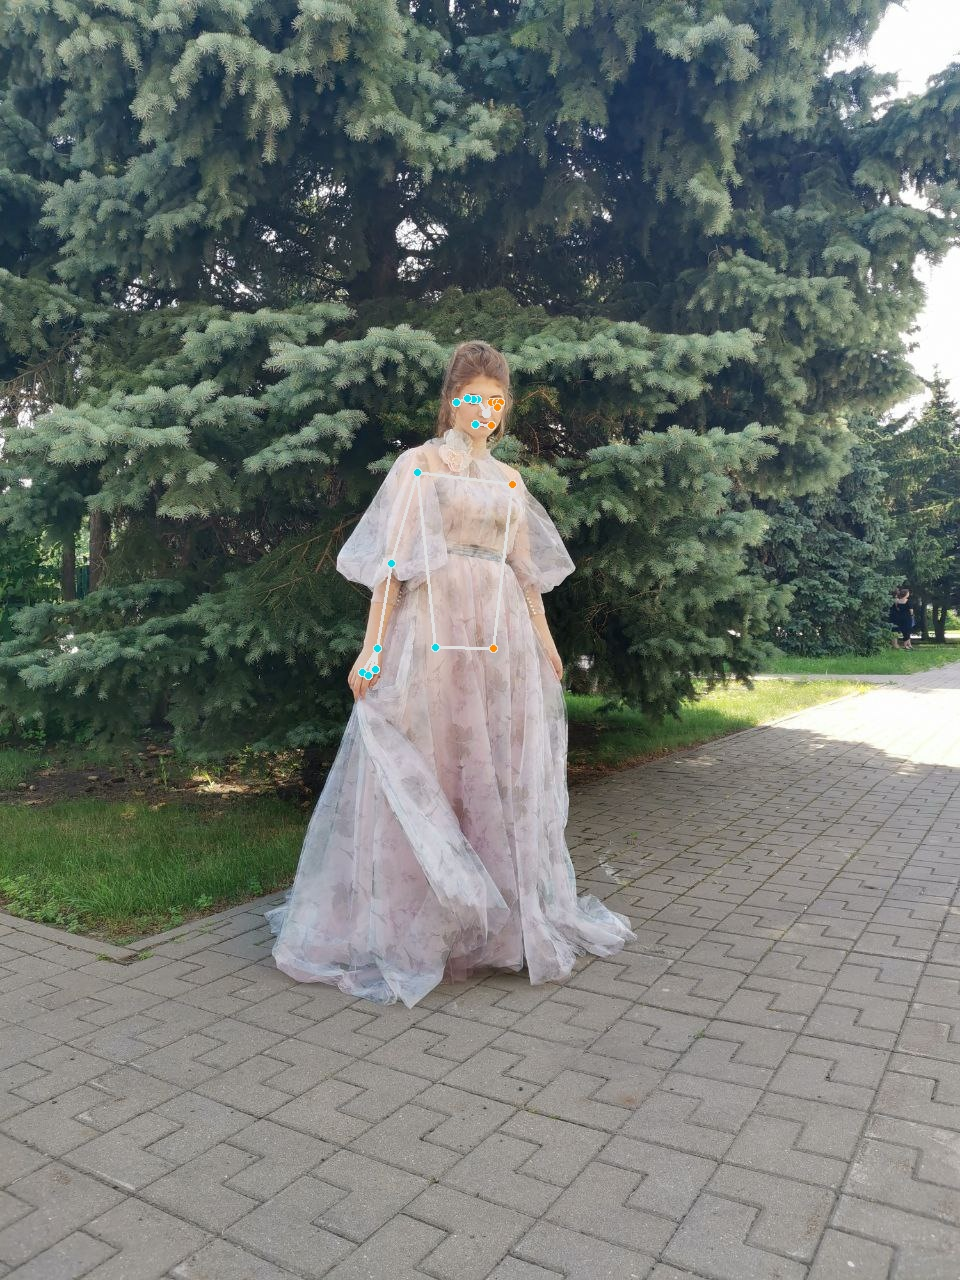
\includegraphics[height=\textwidth]{./images/MPPose/36}
   \caption{ }
\end{subfigure}
\begin{subfigure}[b]{.5\textwidth}
	\centering
   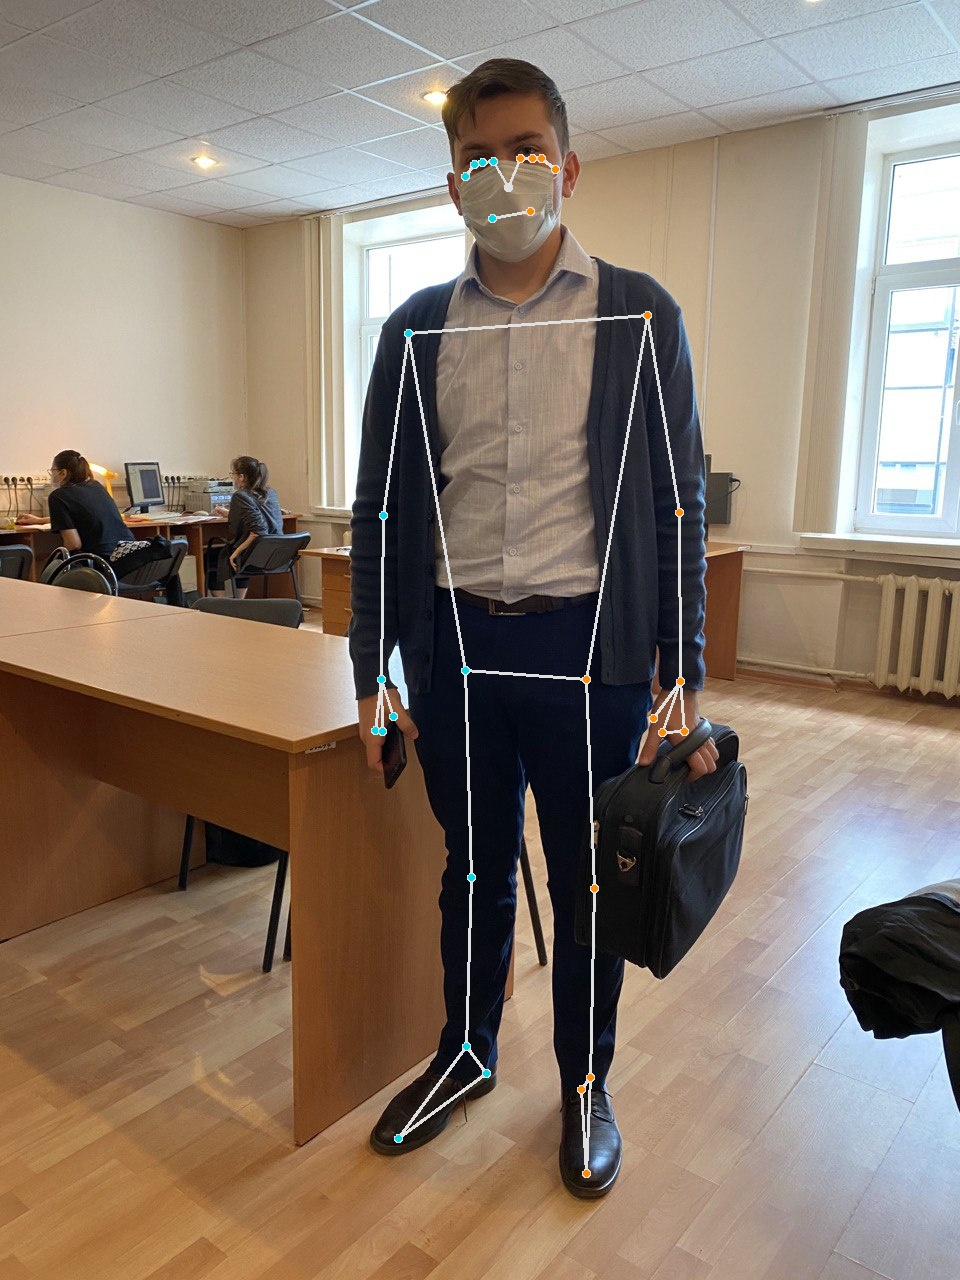
\includegraphics[height=\textwidth]{./images/MPPose/33}
   \caption{ }
\end{subfigure}
   \caption{Пример результатов работы модели BlazePose.}
   \label{fig:MP_result}
\end{figure}

\begin{figure}[h]
\begin{subfigure}[b]{.5\textwidth}
	\centering
	
\includegraphics[width=\textwidth]{./images/MoveNet/19}
	\caption{ }
\end{subfigure}
\begin{subfigure}[b]{.5\textwidth}
	\centering
   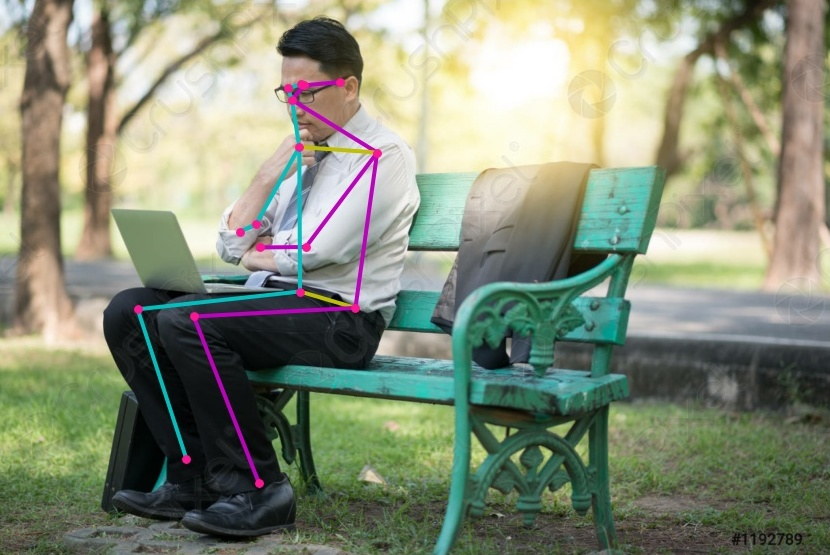
\includegraphics[width=\textwidth]{./images/MoveNet/23}
   \caption{ }
\end{subfigure}
\begin{subfigure}[b]{.5\textwidth}
	\centering
   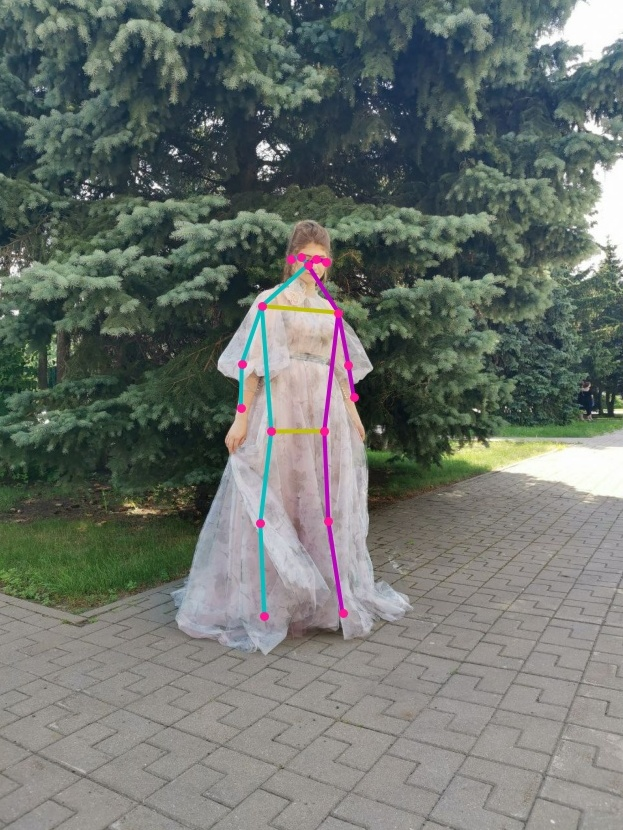
\includegraphics[height=\textwidth]{./images/MoveNet/36}
   \caption{ }
\end{subfigure}
\begin{subfigure}[b]{.5\textwidth}
	\centering
   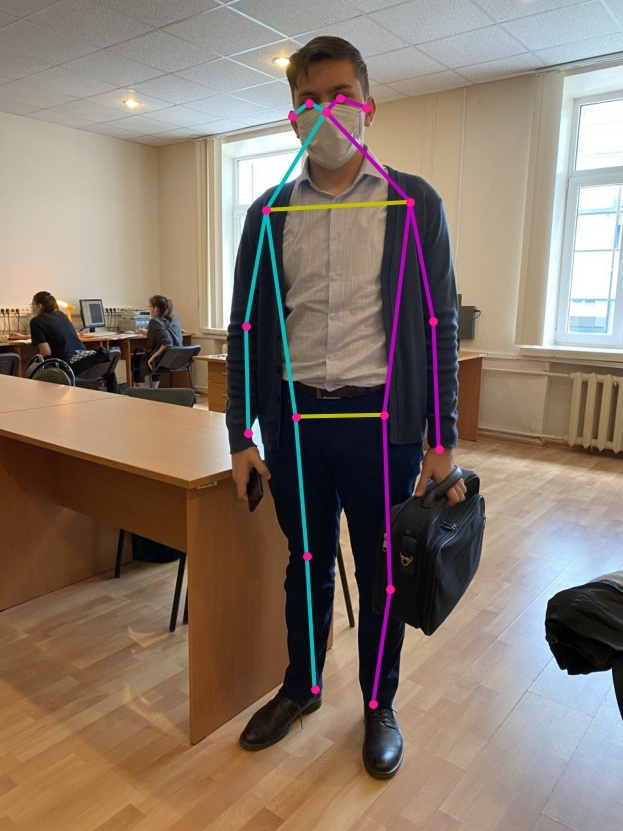
\includegraphics[height=\textwidth]{./images/MoveNet/33}
   \caption{ }
\end{subfigure}
   \caption{Пример результатов работы модели MoveNet.SinglePose.}
   \label{fig:MN_result}
\end{figure}

\begin{figure}[h]
\begin{subfigure}[b]{.5\textwidth}
	\centering
	
\includegraphics[width=\textwidth]{./images/OpenPose/19}
	\caption{ }
\end{subfigure}
\begin{subfigure}[b]{.5\textwidth}
	\centering
   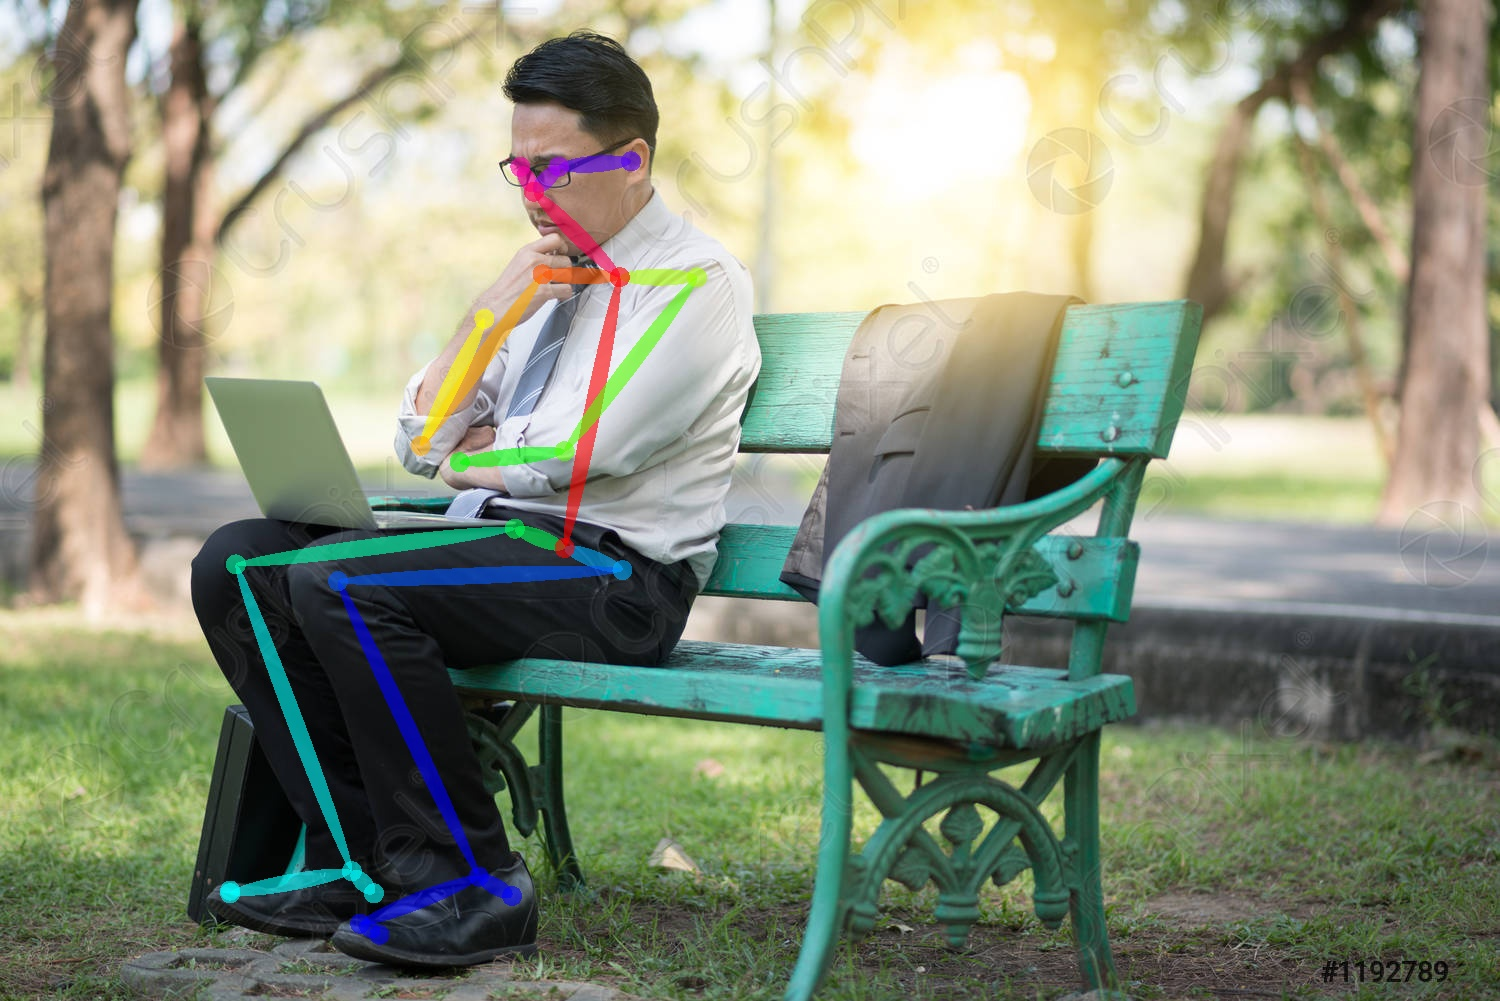
\includegraphics[width=\textwidth]{./images/OpenPose/23}
   \caption{ }
\end{subfigure}
\begin{subfigure}[b]{.5\textwidth}
	\centering
   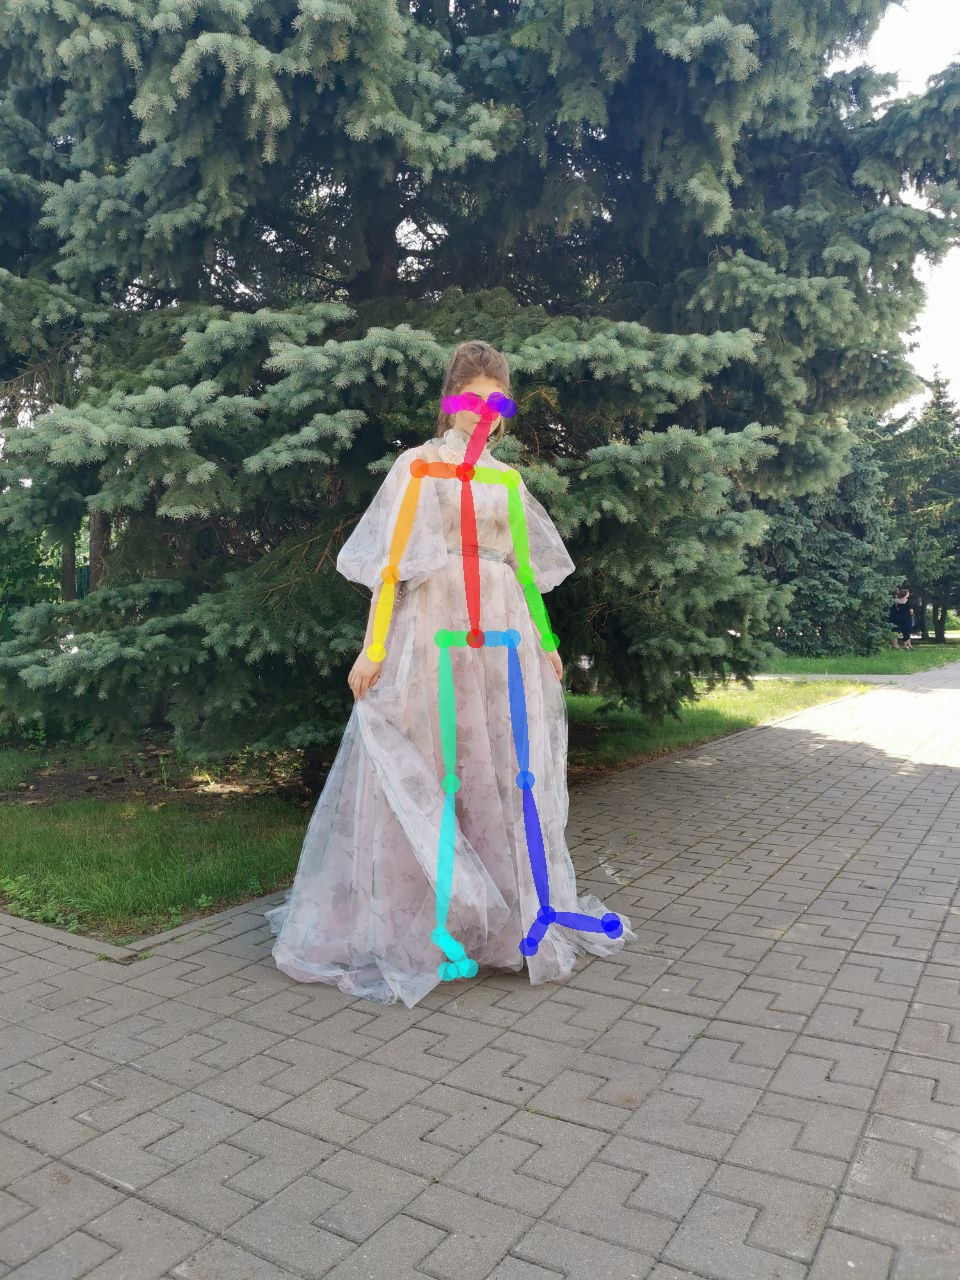
\includegraphics[height=\textwidth]{./images/OpenPose/36}
   \caption{ }
\end{subfigure}
\begin{subfigure}[b]{.5\textwidth}
	\centering
   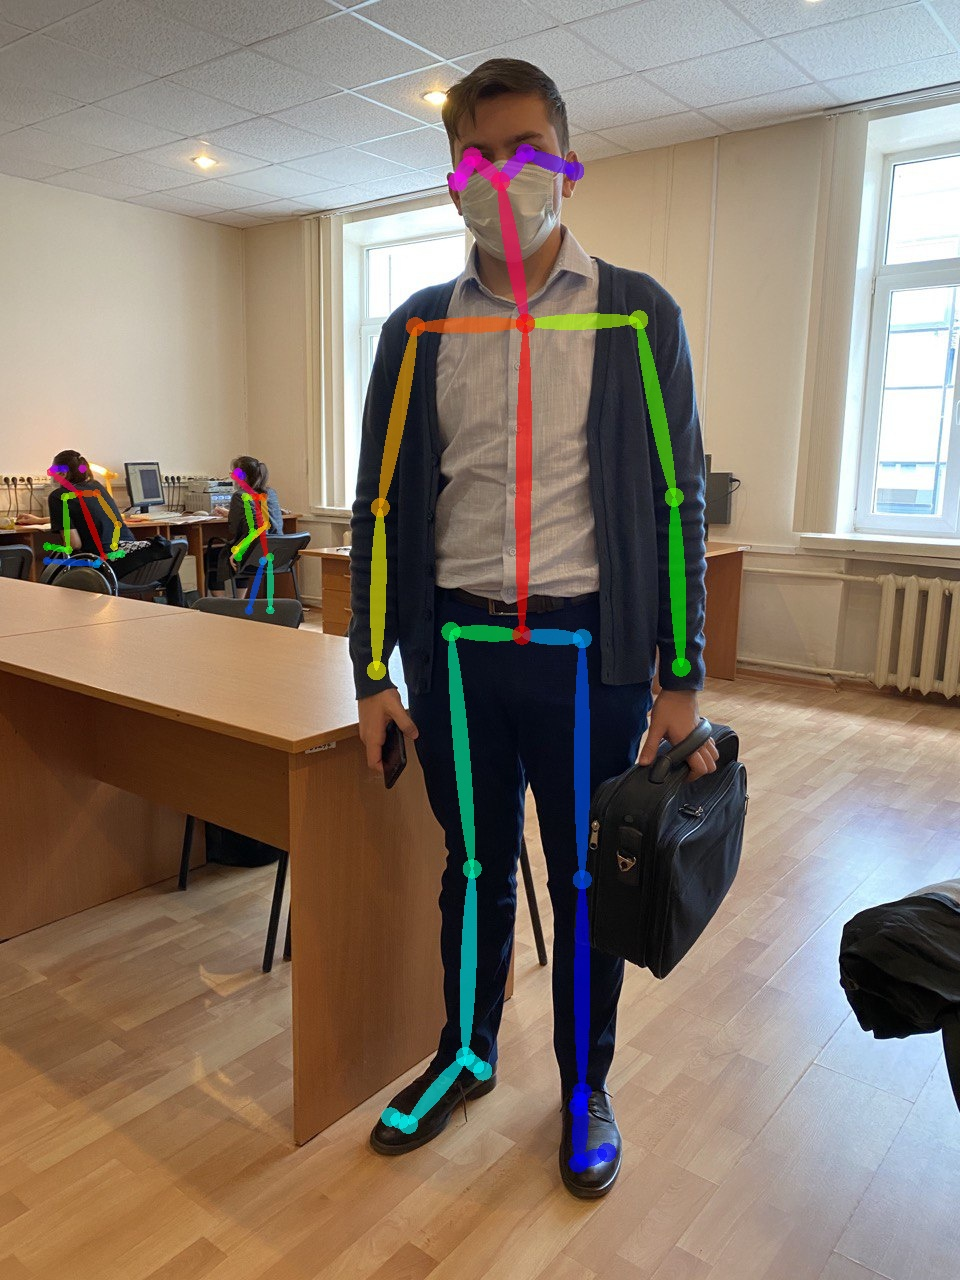
\includegraphics[height=\textwidth]{./images/OpenPose/33}
   \caption{ }
\end{subfigure}
   \caption{Пример результатов работы модели OpenPose.}
   \label{fig:OP_result}
\end{figure}

\begin{figure}[h]
\begin{subfigure}[b]{.5\textwidth}
	\centering
	
\includegraphics[width=\textwidth]{./images/MMPose/19}
	\caption{ }
\end{subfigure}
\begin{subfigure}[b]{.5\textwidth}
	\centering
   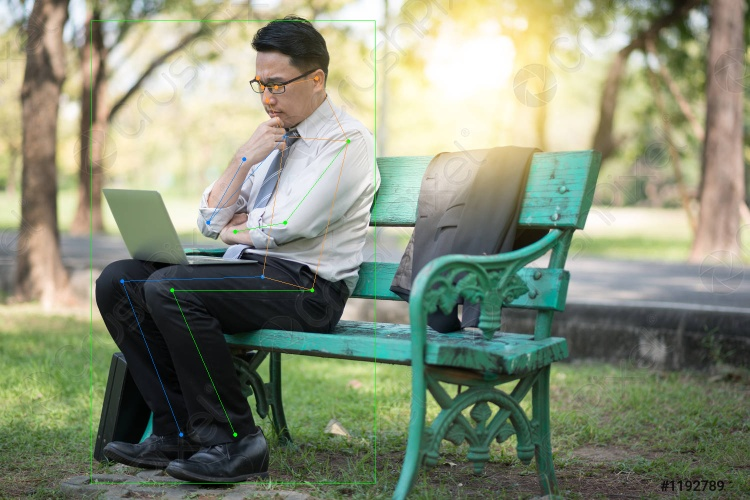
\includegraphics[width=\textwidth]{./images/MMPose/23}
   \caption{ }
\end{subfigure}
\begin{subfigure}[b]{.5\textwidth}
	\centering
   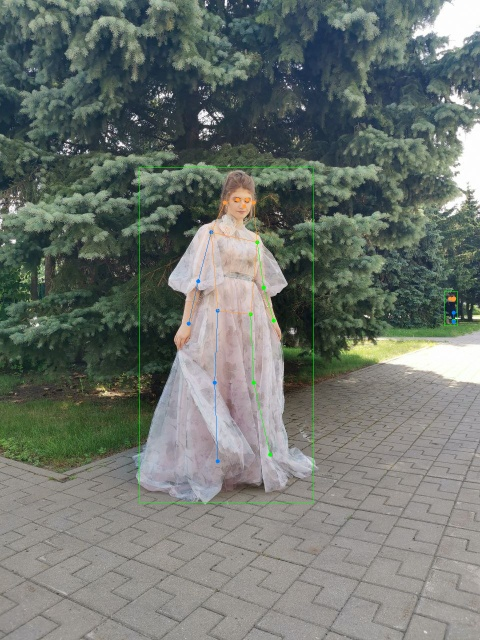
\includegraphics[height=\textwidth]{./images/MMPose/36}
   \caption{ }
\end{subfigure}
\begin{subfigure}[b]{.5\textwidth}
	\centering
   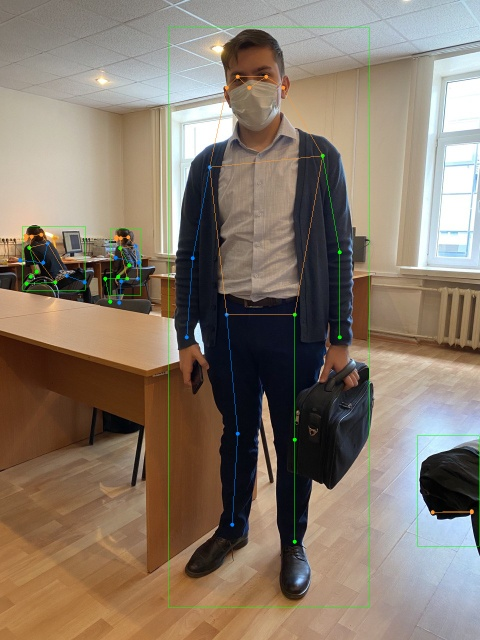
\includegraphics[height=\textwidth]{./images/MMPose/33}
   \caption{ }
\end{subfigure}
   \caption{Пример результатов работы модели MMPose.}
   \label{fig:MMP_result}
\end{figure}
\end{document}